\documentclass{elsarticle}

\usepackage{amsmath}
\usepackage{amsfonts}
\usepackage{mathtools}
\usepackage{cleveref}
\usepackage{bm}
\usepackage{mathrsfs}
\usepackage{placeins}
\usepackage{tcolorbox}
\usepackage{caption}
\usepackage{subcaption}
\usepackage[]{algorithm2e}
\usepackage{amsthm}
\newtcolorbox{satbox}{colback=green!5!white,colframe=green!75!black}
\newtcolorbox{jacbox}{colback=yellow!5!white,colframe=yellow!75!black}
\newtheorem{definition}{Definition}
\newtheorem{remark}{Remark}
\newtheorem{proposition}{Proposition}
\newtheorem{lemma}{Lemma}

%Continuous
\newcommand{\vecs}[1]{\vec{\mskip\thinmuskip #1}}
\newcommand{\wc}{\vecs{w}}
\newcommand{\xic}{\vecs{\xi}}
\newcommand{\wcn}{w_n}
\newcommand{\wct}{w_s}
\newcommand{\uc}{u}
\newcommand{\vc}{v}
\newcommand{\phic}{\vecs{\phi}}
\newcommand{\psic}{\vecs{\psi}}
\newcommand{\nc}{\vecs{n}}
\renewcommand{\div}{{\nabla\cdot}}
\newcommand{\dOmega}{{\partial\Omega}}
\newcommand{\ipc}[2]{\left(#1, #2\right)_\Omega} %Inner product on Omega
\newcommand{\ipbc}[2]{\left(#1, #2\right)_{\partial \Omega}} %Inner product on dOmega
\newcommand{\ipbcpart}[2]{\left(#1, #2\right)_{\Gamma_d}} %Inner product on dOmega
\newcommand{\ipgd}[2]{\left(#1, #2\right)_{\Gamma_d}} %Inner product on Gamma_d
\newcommand{\normc}[1]{\|#1\|_\Omega}


%Discrete
\newcommand{\wn}{\vecs{\bm{w}}}
\newcommand{\wnn}{\bm{w}_n}
\newcommand{\wtn}{\bm{w}_s}
\newcommand{\un}{\bm{u}}
\newcommand{\vn}{\bm{v}}
\newcommand{\pn}{\bm{p}}
\newcommand{\fn}{\bm{f}}
\newcommand{\gn}{\bm{g}}
\newcommand{\en}{\bm{e}}
\newcommand{\xn}{\bm{x}}
\newcommand{\xin}{\vecs{\bm{\xi}}}
\newcommand{\phin}{\vecs{\bm{\phi}}}
\newcommand{\psin}{\vecs{\bm{\psi}}}
\newcommand{\zeron}{\bm{0}}
\newcommand{\In}{\bm{I}}
\newcommand{\nn}{\vecs{\bm{n}}}
\newcommand{\nnx}{\bm{n}_x}
\newcommand{\nny}{\bm{n}_y}
\newcommand{\nablan}{\bm{\nabla}}
\newcommand{\divn}{\bm{\nabla\cdot}}
\newcommand{\Dx}{\bm{D_x}}
\newcommand{\Dy}{\bm{D_y}}
\newcommand{\Pn}{\bm{P}}
\newcommand{\Png}{\bm{P}_d}
\newcommand{\Ln}{\bm{L}}
\newcommand{\Lng}{\bm{L}_d}
\newcommand{\Pncal}{\bm{\mathcal{P}}}
\newcommand{\ipn}[2]{\left(#1, #2\right)_{\Omega_h}} %Discrete inner product on Omega
\newcommand{\normn}[1]{\|#1\|_{\Omega_h}}
\newcommand{\ipbn}[2]{\left(#1, #2\right)_{\Gamma_d}} %Discrete inner product on Gamma
\newcommand{\ipbnfull}[2]{\left(#1, #2\right)_{\partial \Omega_h}} %Discrete inner product on Gamma
\newcommand{\euln}{\bm{\mathcal{L}}}
\newcommand{\satn}{\bm{\mathcal{S}}}
\newcommand{\Hn}{\bm{\mathcal{H}}}
\newcommand{\Fn}{\bm{\mathcal{F}}}
\newcommand{\Mn}{\mathcal{M}}
\newcommand{\diagn}[1]{\underline{#1}}
\newcommand{\soln}{\bm{\chi}}
\newcommand{\cdotn}{\bm{\cdot}}


\title{Explicit Jacobians for the Incompressible Euler Equations on Curvilinear Grids}
\author{Oskar Ålund, Fredrik Laurén, Jan Nordström \\
\it Department of Mathematics, Computational Mathematics, \\
\it Linköping University, \\
\it SE-581 83 Linköping, Sweden\/}
\date{}

\begin{document}
  \begin{abstract}
We derive an explicit form of the Jacobian for discrete approximations of nonlinear initial boundary value problems (IBVPs) on matrix-vector form. The technique is exemplified on the incompressible Navier-Stokes equations in two dimensions. The Jacobian facilitates the use of Newton's method to solve the corresponding nonlinear system of equations. Appropriate boundary conditions are weakly imposed  and we show how to compute the Jacobian for those parts of the discretization as well. The convergence rate of the iterations is verified by using the method of manufactured solutions. The methodology in this paper that can be used on any numerical discretization of IBVPs on matrix-vector form.
\section*{Keywords}
\noindent Nonlinear initial boundary value problems, Jacobian, Newton's method, incompressible Navier-Stokes equations, summation-by-parts, weak boundary conditions.
\end{abstract} 


  \maketitle
  \section{Introduction}%
\label{sec:introduction}

Discretizing partial differential equations revolves around three major considerations:
\begin{enumerate}
  \item Stability
  \item Simplicity
  \item Efficiency
\end{enumerate}
These aspects continually compete for attention, and narrow focus on one of them is often detrimental to the other two. This paper is an attempt to strike a balance between the three in the context of the incompressible Euler equations. Point 1 (stability) is achieved by using well established techniques, such as weakly imposed boundary conditions and integration-by-parts mimicking discrete differential operators. Point 2 (simplicity) is achieved through a convenient notational structure that closely resembles the continuous notation both functionally and visually. Our ambition is to narrow the bridge between the continuous and discrete settings as much as possible so that understanding of the continuous problem transfers with little effort to the discrete problem. Point 3 (efficiency) is achieved using two key tools: encapsulation and explicit Jacobians. By encapsulation we mean that the discrete derivative operators can be thought of as abstract operators that act on discrete approximations of differentiable functions, while satisfying certain key properties (most notably accuracy and summation-by-parts). Such abstraction is useful, not only because it simplifies stability proofs, but also because it isolates concerns: Discrete differentiation can be implemented, optimized, and maintained in separation from any particular solver. Encapsulation also allows us to write down, in very compact form, explicit Jacobians for the discretized incompressible Euler equations in terms of the derivative operators. 

Explicit Jacobians are particularly powerful in the context of implicit timestepping since they are typically orders of magnitude faster to evaluate than for example a finite difference based approximation of the Jacobian. Altough we in this paper consider the incompressible Euler equations in two dimensions, the framework can be extended to any type of hyperbolic or parabolic equations.


  \section{Notation}%
\label{sec:notation}
\begin{figure}
  \begin{subfigure}{.5\textwidth}
    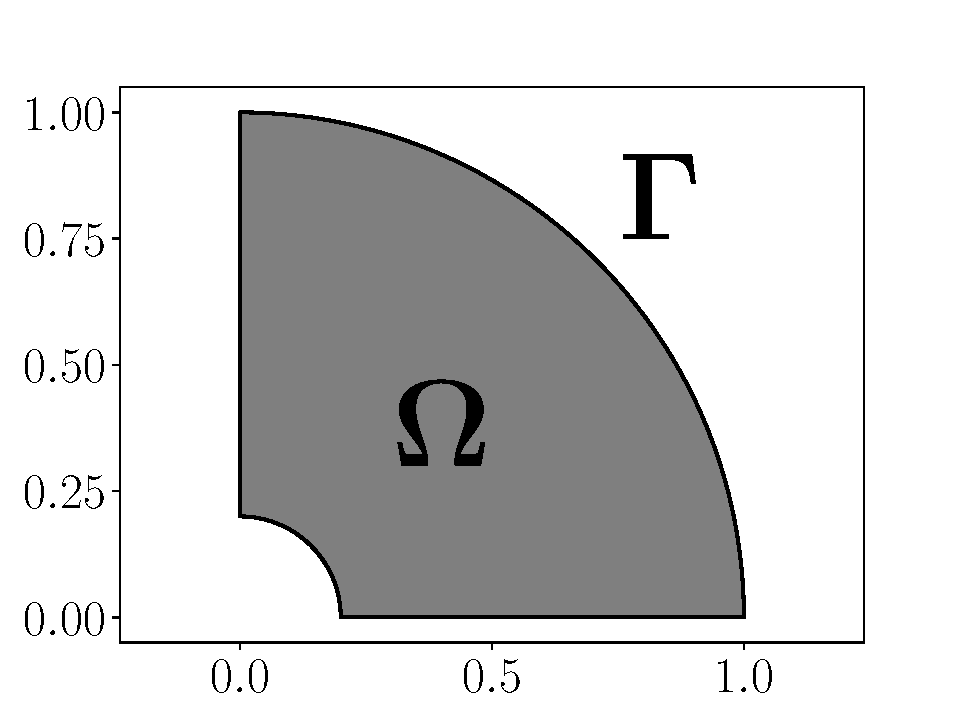
\includegraphics[width=\textwidth]{images/domain.pdf}%
    \caption{An annulus sector domain.}%
    \label{fig:domain}
  \end{subfigure}
  \begin{subfigure}{.5\textwidth}
    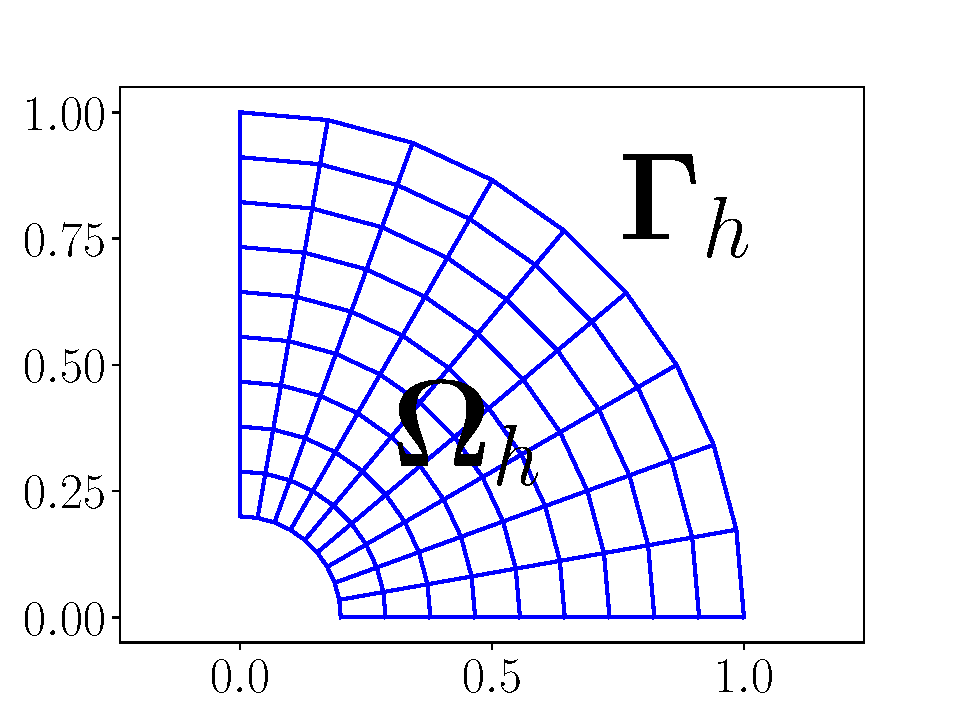
\includegraphics[width=\textwidth]{images/grid.pdf}%
    \caption{A discretization of $\Omega$.}%
    \label{fig:grid}
  \end{subfigure}
  \caption{A curved domain $\Omega$ and a named boundary $\Gamma$.}
\end{figure}
In the continuous setting we consider time dependent scalar- and vector-valued functions on a spatial domain $\Omega$ (such as in Figure~\ref{fig:domain}). Vector-valued functions are column vectors and indicated with an arrow, for example
$
  \vec{w} =
  \begin{pmatrix}
    u & v
  \end{pmatrix}^\top
$
denoting the velocity field. Let $\phic, \psic : \Omega \to \mathbb{R}^n$. We denote by $\normc{\phic}$ and $\ipc{\phic}{\psic}$ the $L^2$ inner product and norm on $\Omega$ respectively,
\begin{equation*}
  \ipc{\phic}{\psic} := \int_\Omega \phic \cdot \psic dx dy \,, \quad \normc{\phic} := \sqrt{\int_\Omega |\phic|^2 dxdy} \,.
\end{equation*}
Similarly, the $L^2$ inner product on $\partial \Omega$ is denoted $\ipbc{\cdot}{\cdot}$,
\begin{equation*}
  \ipbc{\phic}{\psic} := \int_{\partial \Omega} \phic \cdot \psic ds \,.
\end{equation*}
Recall the definitions of the gradient ($\nabla$) and divergence ($\div$) operators,
\begin{equation*}
  \nabla u = (u_x, u_y), \quad \div\wc = u_x + v_y \,,
\end{equation*}
and Green's identity,
\begin{equation}
  \label{eq:greens_identity}
  \ipc{\phic}{\nabla\psi} = \ipbc{\phic \cdot \nc}{\psi} - \ipc{\div \phic}{\psi} \,.
\end{equation}
where $\nc$ is the outward point unit normal of the boundary $\partial \Omega$. We allow the gradient, the divergence, and the dot product to operate row-wise, so that for example
\begin{equation*}
  \wc \cdot \nabla \wc =
  \begin{pmatrix}
    \wc \cdot \nabla u \\
    \wc \cdot \nabla v
  \end{pmatrix}
  =
  \begin{pmatrix}
    u u_x + v u_y \\
    u v_x + v v_y
  \end{pmatrix}
\end{equation*}
and
\begin{equation*}
  \div \wc \wc^\top =
  \div
  \begin{pmatrix}
    uu & uv \\
    uv & vv
  \end{pmatrix}
  =
  \begin{pmatrix}
    {(uu)}_x + {(uv)}_y \\
    {(uv)}_x + {(vv)}_y
  \end{pmatrix} \,.
\end{equation*}

The semi-discrete setting mimics the continuous setting to a large extent, with a few caveats (such as no product rule for differentiation). Notationally we will see that the continuous and discrete settings are virtually identical.

Consider an $N_x$-by-$N_y$ curvilinear grid $\Omega_h$ as in Figure~\ref{fig:grid}. We think of our semi-discrete solutions as column vectors of function evaluations on this grid, denoted in bold. For example, if
$
  u : \Omega \to \mathbb{R}
$,
then
$
  \un =
  \begin{pmatrix}
    \un_1^\top & \un_2^\top & \cdots & \un_{N_x}^\top
  \end{pmatrix}^\top
$,
where
\[
  \un_i =
  \begin{pmatrix}
    u_{i1} & u_{i2} & \cdots & u_{iN_y}
  \end{pmatrix}^\top
  \approx
  \begin{pmatrix}
    u(x_{i1}, y_{i1}) & u(x_{i2}, y_{i2}) & \cdots & u(x_{iN_y}, y_{iN_y})
  \end{pmatrix}^\top \,.
\]

Note that $\un$ is a special kind of vector in that its purpose is to approximate a continuous function. To make this distinction clear let us make a formal definition.

\begin{definition}
  Given an $N_x$-by-$N_y$ curvilinear grid $\Omega_h$, a vector $\un \in \mathbb{R}^{N_x N_y}$ is called a \emph{grid function}.
\end{definition}

We make extensive use of elementwise operations on grid functions. If $\un$ and $\vn$ are grid functions, then the elementwise product is indicated with no symbol,
\begin{equation*}
  \un\vn =
  \begin{pmatrix}
    u_{11}v_{11} & u_{12}v_{12} & \cdots & u_{21}v_{21} & u_{22}v_{22} & \cdots
  \end{pmatrix}^\top \,.
\end{equation*}
Similarly elementwise fractions are indicated by a division symbol,
\begin{equation*}
  \un/\vn =
  \begin{pmatrix}
    u_{11}/v_{11} & u_{12}/v_{12} & \cdots & u_{21}/v_{21} & u_{22}/v_{22} & \cdots
  \end{pmatrix}^\top \,.
\end{equation*}
For a scalar function $h : \mathbb{R} \to \mathbb{R}$ we will write $h(\un)$ to indicate elementwise application of $h$ to $\un$,
\begin{equation*}
  h(\un) =
  \begin{pmatrix}
    h(u_{11}) & h(u_{12}) & \cdots & h(u_{21}) & h(u_{22}) & \cdots
  \end{pmatrix}^\top \,.
\end{equation*}

To further mimic the continuous setting we introduce matrices with grid function components. To get a sense for what this means and why it is useful, let us consider an example. In the incompressible Euler equations, the outer product
\begin{equation*}
  \wc \wc^\top =
  \begin{pmatrix}
    uu & uv \\
    uv & vv
  \end{pmatrix}
\end{equation*}
appears (see equation~\eqref{eq:euler_nobc_split} in Section~\ref{sec:euler}). To mimic this operation it is not enough to simply concatenate grid functions into a long vector. Consider what happens if we multiply the vectors
$
\begin{pmatrix}
  \un^\top & \vn^\top
\end{pmatrix}^\top
$
and
$
\begin{pmatrix}
  \un^\top & \vn^\top
\end{pmatrix}
$. The result is an $N_x N_y$-by-$N_x N_y$ matrix that does not correspond to any sort of approximation of $\wc \wc^\top$. Instead, we need to be able to form matrices where the components of the matrices are not scalars, but grid functions. Such matrices will be denoted by square brackets, and their transposes by $\dagger$. For example, the discrete velocity field is
\begin{equation*}
  \wn =
  \begin{bmatrix}
    \un \\ \vn
  \end{bmatrix}
\end{equation*}
and its transpose is
$
\wn^\dagger =
\begin{bmatrix}
  \un & \vn
\end{bmatrix}
$. Note that transposition \emph{does not} act on the individual grid functions of the matrix. This means that when we form the outer product
\begin{equation*}
  \wn \wn^\dagger =
  \begin{bmatrix}
    \un \un & \un \vn \\
    \un \vn & \vn \vn
  \end{bmatrix}
\end{equation*}
we get a matrix that approximates $\wc \wc^\top$.

A column matrix of grid functions, like $\wn$, is called a \emph{vector valued} grid function. We define the dot product between two vector valued grid functions
$
  \phin =
  \begin{bmatrix}
    \bm{\phi}_1 & \bm{\phi}_2 & \cdots & \bm{\phi}_n
  \end{bmatrix}^\dagger
$
and
$
  \psin =
  \begin{bmatrix}
    \bm{\psi}_1 & \bm{\psi}_2 & \cdots & \bm{\psi}_n
  \end{bmatrix}^\dagger
$
as
\begin{equation*}
  \phin \cdotn \psin = \phin^\dagger \psin = \sum_{i=1}^n \bm{\phi}_i \bm{\psi}_i \,.
\end{equation*}
Note that if $\phin$ and $\psin$ approximate the vector valued functions $\phic$ and $\psic$, then $\phin \cdot \psin$ is a grid function that approximates the scalar function $\phic \cdot \psic$.

For numerical differentiation we use the encapsulated SBP operators described in~\cite{aalund2019encapsulated}, together with some additional convenient notation. Let $\Dx$ and $\Dy$ be encapsulated SBP operators on $\Omega_h$ in the $x$- and $y$-direction respectively. Associated with the operators $\Dx$ and $\Dy$ is a diagonal positive definite quadrature matrix $\Pn$. This matrix defines a discrete inner product and a norm:
\begin{equation*}
  \ipn{\un}{\vn} := \un^\top \Pn \vn \approx \ipc{u}{v}, \quad
  \|\un\|_{\Omega_h} := \sqrt{\ipn{\un}{\un}} \approx \|u\|_{\Omega} \,.
\end{equation*}
The above norm and inner product have natural extensions to vector valued grid functions:
\begin{equation*}
  \ipn{\phin}{\psin} := \sum_{i=1}^n \ipn{\bm{\phi}_i}{\bm{\psi}_i}, \quad
  \normn{\phin} := \sqrt{\sum_{i=1}^n \normn{\bm{\phi}_i}^2} \,.
\end{equation*}
We refer to the operation
$
  \ipn{\cdotn}{\cdotn}
$
as \emph{discrete integration in space}.

Consider now $\Gamma_d$, $d \in \{e,w,s,n\}$---the four boundaries of $\Omega_h$. Also associated with the SBP operators are the numerical outward-pointing normals of $\Gamma_d$:
$
  \nn =
  \begin{bmatrix}
    \nnx & \nny
  \end{bmatrix}^\dagger
$,
as well as diagonal boundary quadrature matrices $\Pn_d$. The matrix $\Pn_d$ defines a discrete inner product on the boundary $\Gamma_d$:
\[
  \ipbn{\un}{\vn} := \un^\top \Pn_d \vn \approx \int_{\Gamma_d} uv ds \,.
\]
We also define the discrete inner product on the full boundary $\partial \Omega_h$:
\[
  \ipbnfull{\un}{\vn} := \sum_d \ipbn{\un}{\vn} \approx \int_{\partial \Omega} uv ds \,.
\]

Recall from~\cite{aalund2019encapsulated} that the operators $\Dx$ and $\Dy$ satisfy the following summation-by-parts properties.
\begin{proposition}%
  \label{prop:sbp}
  Assume $\Dx$ and $\Dy$ are SBP operators on a curvilinear grid $\Omega_h$, and $\un$, $\vn$ are grid functions. Then
  \begin{align*}
    \ipn{\un}{\Dx \vn} &= \ipbnfull{\un}{\nnx \vn} - \ipn{\Dx \un}{\vn} \,, \\
    \ipn{\un}{\Dy \vn} &= \ipbnfull{\un}{\nny \vn} - \ipn{\Dy \un}{\vn} \,.
  \end{align*}
\end{proposition}

\begin{remark}
  Proposition~\ref{prop:sbp} is a discrete version of the integration by parts formulas $\ipc{u}{v_x} = \ipbc{u}{n_x v} - \ipc{u_x}{v}$ and $\ipc{u}{v_y} = \ipbc{u}{n_y v} - \ipc{u_y}{v}$.
\end{remark}

We define the discrete gradient $\nablan$ and divergence $\divn$ by
\begin{align*}
  \nablan \un &:=
  \begin{bmatrix}
    \Dx \un & \Dy \un
  \end{bmatrix} \\
  \divn \wn &:= \Dx \un + \Dy \vn \,.
\end{align*}
These operators may also act row-wise on matrices just like in the continuous setting, so that for example
\begin{align*}
  \wn \cdotn \nablan \wn =
  \begin{bmatrix}
    \wn \cdotn \nablan \un \\
    \wn \cdotn \nablan \vn
  \end{bmatrix}
  =
  \begin{bmatrix}
    \un \Dx \un + \vn \Dy \un \\
    \un \Dx \vn + \vn \Dy \vn
  \end{bmatrix}
\end{align*}
and
\begin{align*}
  \divn \wn\wn^\dagger =
  \divn
  \begin{bmatrix}
    \un\un & \un\vn \\
    \un\vn & \vn\vn
  \end{bmatrix}
  =
  \begin{bmatrix}
    \Dx(\un\un) + \Dy(\un\vn) \\
    \Dx(\un\vn) + \Dy(\vn\vn)
  \end{bmatrix} \,.
\end{align*}

A discrete version of Green's identity follows directly from Proposition~\ref{prop:sbp}.

\begin{proposition}%
  \label{prop:discrete_greens_identity}
  Assume $\Dx$ and $\Dy$ are encapsulated SBP operators on a curvilinear grid $\Omega_h$, $\phin$ is a vector-valued grid function with two compoments, and $\bm{\psi}$ is a grid function. Then
  \begin{equation*}
    \ipn{\phin}{\nablan \bm{\psi}} = \ipbnfull{\phin \cdotn \nn}{\bm{\psi}} - \ipn{\divn \phin}{\bm{\psi}} \,.
  \end{equation*}
\end{proposition}
\begin{proof}
  By Proposition~\ref{prop:sbp},
  \begin{align*}
    \ipn{\phin}{\nablan \bm{\psi}}
      &= \ipn{\bm{\phi}_1}{\Dx \bm{\psi}} + \ipn{\bm{\phi}_2}{\Dy \bm{\psi}} \\
      &= \ipbnfull{\bm{\phi}_1}{\nnx \bm{\psi}} - \ipn{\Dx \bm{\phi}_1}{\bm{\psi}} + \ipbnfull{\bm{\phi}_2}{\nny \bm{\psi}} - \ipn{\Dy \bm{\phi}_2}{\bm{\psi}} \\
      &= \ipbnfull{\bm{\phi}_1}{\nnx \bm{\psi}} + \ipbnfull{\bm{\phi}_2}{\nny \bm{\psi}} - \ipn{\Dx \bm{\phi}_1 + \Dy \bm{\phi}_2}{\bm{\psi}} \\
      &= \ipbnfull{\phin \cdotn \nn}{\bm{\psi}} - \ipn{\divn \phin}{\bm{\psi}} \,.
  \end{align*}
\end{proof}

  \section{The incompressible Euler equations}%
\label{sec:euler}
Consider the incompressible Euler equations
\begin{subequations}%
\label{eq:euler_nobc}
  \begin{align}
    \wc_t + \wc \cdot \nabla \wc &= -\nabla p \label{eq:continuous_euler1} \\
    \div \wc &= 0 \label{eq:div_zero}
  \end{align}
\end{subequations}
where
$
  \wc =
  \begin{bmatrix}
    \uc & \vc
  \end{bmatrix}^\top
$
is the velocity field, $p$ is the pressure. The form~\eqref{eq:continuous_euler1} is not suitable for discretization because its energy analysis relies on the chain rule, which cannot be replicated discretely. Let us go through the energy analysis to see that it does indeed rely on the chain rule (this will also help us understand how to get around the problem).

The rate of change in the kinetic energy $\frac{1}{2}\normc{\wc}^2$ can be found by multiplying~\eqref{eq:continuous_euler1} by $2\wc^\top$ and integrating in space, since
\[
  2\ipc{\wc}{\wc_t} = \frac{d}{dt} \|\wc\|_\Omega^2 \,.
\]
The convective term $\wc \cdot \nabla \wc$ adds or dissipates energy through the boundaries via the integral
$
  2\ipc{\wc}{\wc \cdot \nabla \wc}
$.
Let $\wcn = \wc \cdot \nc$ (the normal velocity). An expression for the energy rate of change due to convection can be derived as follows.
\begin{lemma}\label{lemma:convection1}
  The incompressible Euler equations~\eqref{eq:euler_nobc} imply that
  \begin{equation*}
    2\ipc{\wc}{\wc \cdot \nabla \wc} = \ipbc{\wcn}{|\wc|^2} \,.
  \end{equation*}
\end{lemma}
\begin{proof}
  \begin{align*}
    2\ipc{\wc}{\wc \cdot \nabla \wc}
      &= 2\ipc{u}{\wc \cdot \nabla u} + 2\ipc{v}{\wc \cdot \nabla v} \\
      &= \ipc{\wc}{\nabla u^2} + \ipc{\wc}{\nabla v^2} &&\text{(Chain rule)} \\
      &= \ipc{\wc}{\nabla |\wc|^2} \\
      &= \ipbc{\wcn}{|\wc|^2} - \ipc{\div \wc}{|\wc|^2} &&\text{(Green's identity)} \\
      &= \ipbc{\wcn}{|\wc|^2} &&\text{(Zero divergence)}\,.
  \end{align*}
\end{proof}

Using Lemma~\ref{lemma:convection1} it is straightforward to write $ \frac{d}{dt} \normc{\wc}^2$ in terms of boundary contributions.
\begin{proposition}\label{prop:energy1}
  The incompressible Euler equations~\eqref{eq:euler_nobc} imply that
  \begin{equation*}
    \frac{d}{dt} \normc{\wc}^2 = -\ipbc{\wcn}{|\wc|^2} - 2\ipbc{\wcn}{p}\,.
  \end{equation*}
\end{proposition}
\begin{proof}
  \begin{align*}
    \frac{d}{dt} \normc{\wc}^2
      &= -2\ipc{\wc}{\wc \cdot \nabla \wc} - 2\ipc{\wc}{\nabla p} \\
      &= -\ipbc{\wcn}{|\wc|^2} - 2\ipc{\wc}{\nabla p} &&\text{(Lemma~\ref{lemma:convection1})} \\
      &= -\ipbc{\wcn}{|\wc|^2} - 2\ipbc{\wcn}{p} + 2\ipc{\div \wc}{p} &&\text{(Green's identity)} \\
      &= -\ipbc{\wcn}{|\wc|^2} - 2\ipbc{\wcn}{p} &&\text{(Zero divergence)} \\
  \end{align*}
\end{proof}

We want to remove the dependence on the chain rule in the energy analysis. To this end, note that the identity
$
  \div (\wc \wc^\top) = \wc \div \wc + \wc \cdot \nabla \wc = \wc \cdot \nabla \wc
$
holds since $\div \wc = 0$. Hence, the incompressible Euler equations  can be rewritten in split form as
\begin{subequations}%
\label{eq:euler_nobc_split}
  \begin{align}
    \wc_t + \frac{1}{2} \wc \cdot \nabla \wc + \frac{1}{2} \div (\wc \wc^\top) &= -\nabla p \label{eq:continuous_euler2} \\
    \div \wc &= 0 \,. \label{eq:div_zero2}
  \end{align}
\end{subequations}
The energy analysis for~\eqref{eq:euler_nobc_split} can then be performed without the chain rule by using the following lemma.

\begin{lemma}\label{lemma:convection2}
  For any smooth $\wc : \Omega \to \mathbb{R}^2$,
  \begin{equation*}
    \ipc{\wc}{\wc \cdot \nabla \wc} = \ipbc{\wcn}{|\wc|^2} - \ipc{\wc}{\div (\wc \wc^\top)} \,.
  \end{equation*}
\end{lemma}

\begin{proof}
  \begin{align*}
    \ipc{\wc}{\wc \cdot \nabla \wc}
      &= \ipc{u}{\wc \cdot \nabla u} + \ipc{v}{\wc \cdot \nabla v} \\
      &= \ipc{u\wc}{\nabla u} + \ipc{v\wc}{\nabla v} \\
      &= \ipbc{u\wcn}{u} - \ipc{\div (u\wc)}{u} + \ipbc{v\wcn}{v} - \ipc{\div (v\wc)}{v} \\
      &= \ipc{\wcn}{u^2+v^2} - \ipc{u}{\div (u\wc)} - \ipc{v}{\div (v\wc)} \\
      &= \ipbc{\wcn}{|\wc|^2} - \ipc{u}{\div (u\wc)} - \ipc{v}{\div (v\wc)} \\
      &= \ipbc{\wcn}{|\wc|^2} - \ipc{\wc}{\div (\wc \wc^\top)} \,.
  \end{align*}
  In the above equalities we have only used Green's identity and the definitions of the inner products.
\end{proof}
Finally we restate Proposition~\ref{prop:energy1} for the split form incompressible Euler equations~\eqref{eq:euler_nobc_split}, and prove it without reference to the chain rule.

\begin{proposition}\label{prop:energy2}
   The split form incompressible Euler equations~\eqref{eq:euler_nobc_split} imply that
  \begin{equation*}
    \frac{d}{dt} \normc{\wc}^2 = -\ipbc{\wcn}{|\wc|^2} - 2\ipbc{\wcn}{p}\,.
  \end{equation*}
\end{proposition}

\begin{proof}
  \begin{align*}
    \frac{d}{dt} \normc{\wc}^2
      &= -\ipc{\wc}{\wc \cdot \nabla \wc} -\ipc{\wc}{\div (\wc \wc^\top)} - 2\ipc{\wc}{\nabla p} \\
      &= -\ipbc{\wcn}{|\wc|^2} - 2\ipc{\wc}{\nabla p} &&\text{(Lemma~\ref{lemma:convection2})} \\
      &= -\ipbc{\wcn}{|\wc|^2} - 2\ipbc{\wcn}{p} + 2\ipc{\div \wc}{p} &&\text{(Green's identity)} \\
      &= -\ipbc{\wcn}{|\wc|^2} - 2\ipbc{\wcn}{p} &&\text{(Zero divergence)} \\
  \end{align*}
\end{proof}

\begin{remark}
  The proof of Proposition~\ref{prop:energy2} relies only on properties that can be replicated discretely, namely Green's identity and algebraic properties of the inner product. In fact, as we shall see in Section~\ref{sec:discretization}, the energy analysis of our discretization of the split form incompressible Euler equations~\eqref{eq:euler_nobc_split} is identical to the proofs of Lemma~\ref{lemma:convection2} and Proposition~\ref{prop:energy2}.
\end{remark}

If the boundary terms in Proposition~\ref{prop:energy2} can be bounded in terms of data, then a bound on the kinetic energy can be found at any given time in terms of initial and boundary data.

\begin{proposition}\label{prop:kinetic_energy_bound}
 Assume that $\wc$ and $p$ are smooth solutions to~\eqref{eq:euler_nobc_split} and that  $\wc = \vecs{f}$ for $t=0$, where $\vecs{f}$ is the initial data.
 Furthermore, assume that $-\ipbc{\wcn}{|\wc|^2} - 2\ipbc{\wcn}{p} = g$. Then for $T > 0$,
  \begin{equation*}
    \normc{\wc}^2(T) = \normc{\vecs{f}}^2 + \int_0^T g(t) dt \,.
  \end{equation*}
\end{proposition}

\begin{proof}
  By Proposition~\ref{prop:energy2},
  \begin{equation*}
    \int_0^T \frac{d}{dt} \normc{\wc}^2dt = \normc{\wc}^2(T) - \normc{\wc}^2(0) = \int_0^T g(t) dt \,.
  \end{equation*}
  Hence,
  \begin{equation*}
    \normc{\wc}^2(T) = \normc{\vecs{f}}^2 + \int_0^T g(t) dt \,.
  \end{equation*}
\end{proof}


  \section{Boundary conditions}%
\label{sec:boundary_conditions}
A number of different boundary conditions can be used for various modeling goals. Below we list the ones that are used in this paper. We select, for each of the four boundaries $\Gamma_d$ of $\Omega$, one of the conditions listed below. All conditions (except for the inflow condition in Section~\ref{sec:continuous_inflow}) are built to either dissipate or conserve kinetic energy. More precisely, we choose to impose boundary conditions at $\Gamma_d$ which lead to
\begin{equation}
  \label{eq:energy_gamma_d}
  -\ipbcpart{\wcn}{|\wc|^2} - 2\ipbcpart{\wcn}{p} \leq 0 \,.
\end{equation}
Note that
\begin{equation*}
  \ipbc{\wcn}{|\wc|^2} + 2\ipbc{\wcn}{p} = \sum_d \left(\ipbcpart{\wcn}{|\wc|^2} + 2\ipbcpart{\wcn}{p} \right) \,.
\end{equation*}
Hence, if~\eqref{eq:energy_gamma_d} is satisfied for all four boundaries, Proposition~\ref{prop:kinetic_energy_bound} implies that the kinetic energy does not grow.

As we shall see in Section~\ref{sec:discrete_boundary_conditions}, the continuous bounds are mimicked in the discrete setting by using encapsulated SBP operators and weakly imposed boundary conditions.

\subsection{Solid wall}
To model a solid wall we may impose vanishing normal velocity, $\wcn = 0$, so that the boundary terms in~\eqref{eq:energy_gamma_d} cancel. Figure~\ref{fig:cavity_flow} shows a simulation of a cavity flow using this boundary condition on the entire boundary $\partial \Omega$.
\begin{figure}%
  \centering
  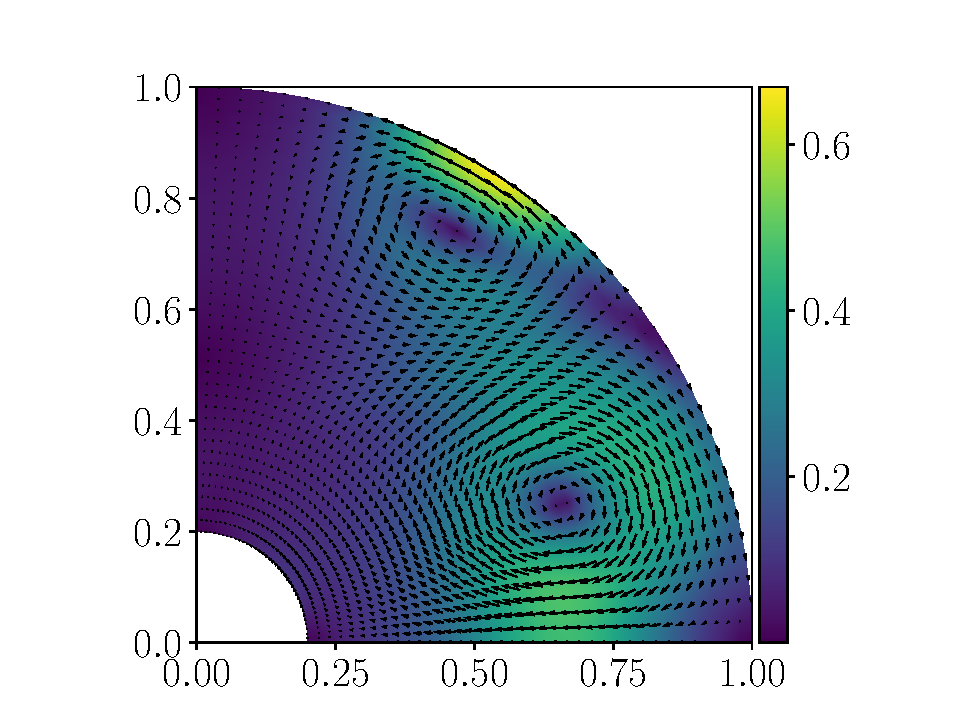
\includegraphics[width=0.7\textwidth]{images/cavity_flow.pdf}
  \caption{Flow inside an annulus sector with the boundary condition $\wcn = 0$ imposed on all four boundaries.}%
  \label{fig:cavity_flow}
\end{figure}

\subsection{Pressure outflow}\label{sec:pressure_outflow}
If $\wcn > 0$  on $\Gamma_d$ it suffices to specify the pressure $p$. Indeed, if $\wcn > 0$ and a nonnegative pressure $p$ is imposed, then $-\ipbcpart{\wcn}{|\wc|^2} - 2\ipbcpart{\wcn}{p} \leq 0$. This can be used to model a priori known outflow boundaries, for example a horizontal flow inside a channel (see Figure~\ref{fig:bump_flow}).

\subsection{Stabilized pressure outflow}%
\label{sub:stab_pressure}
Only prescribing the pressure as described in Section~\ref{sec:pressure_outflow} will lead to instability if the boundary changes from an outflow to an inflow, since $-\ipgd{\wcn}{|\wc|^2} - 2\ipgd{\wcn}{p} > 0$ if $\wcn < 0$. Consider instead the boundary condition
\begin{equation}
  \begin{aligned}
    h(\wcn) \wcn^2 + 2p & = 0
    \\
    h(\wcn) \wct^2 & = 0
  \end{aligned}
  \quad \quad \text{where} \quad
  h(\wcn) =
  \begin{cases}
     1 \quad \text{if} \quad \wcn < 0
     \\
     0 \quad \text{if} \quad \wcn \ge 0
  \end{cases}
  \,.
  \label{eq:stabilized_outflow}
\end{equation}
Here, $\wct = -n_y u + n_x v$ is the tangential velocity. If $\wcn \geq 0$, then~\eqref{eq:stabilized_outflow} is reduced to the pressure outflow condition. If $\wcn < 0$, then the condition $\wcn^2 + p = 0$ serves to attract the fluid since it decreases the pressure at the boundary, while the condition $\wct = 0$ restricts tangential flow (see Figure~\ref{fig:stab_pressure}). Furthermore, if $\wcn < 0$, imposing~\eqref{eq:stabilized_outflow} on $\Gamma_d$ yields
\begin{equation*}
  -\ipbcpart{\wcn}{|\wc|^2} - 2\ipbcpart{\wcn}{p} = -\ipbcpart{\wcn}{\wcn^2 + \wct^2 + 2p} = 0 \,.
\end{equation*}

\begin{figure}%
  \centering
  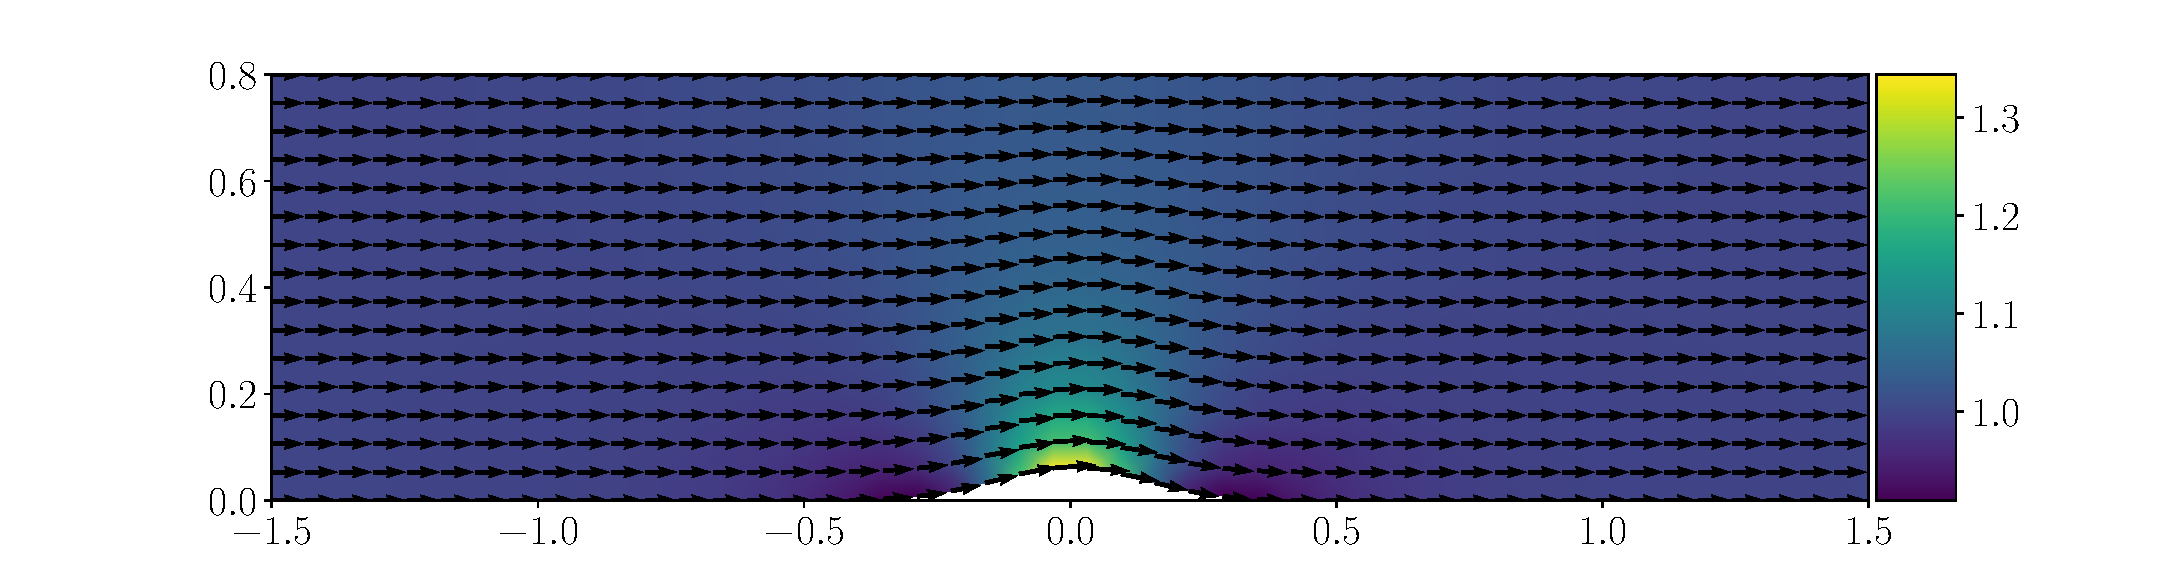
\includegraphics[width=\textwidth]{images/bump_flow.pdf}
  \caption{Flow inside a channel with a bump.}%
  \label{fig:bump_flow}
\end{figure}

\subsection{Inflow}\label{sec:continuous_inflow}
To model an inflow boundary we may impose the conditions $\wcn = g_n$ and $\wct = g_s$, specifying the normal and tangential velocity. Note that this implies that
\begin{equation*}
  -\ipbcpart{\wcn}{|\wc|^2} - 2\ipbcpart{\wcn}{p} = -\ipbcpart{g_n}{g_n^2 + g_s^2} - 2\ipbcpart{g_n}{p} \,,
\end{equation*}
which is only bounded in terms of data under the assumption that $p$ is bounded. To the best of our knowledge, there is no proof that $p$ is bounded. Our numerical experiments do not exhibit any issues related to uncontrolled growth in $p$, but the inflow boundary condition should still be used with care since there is no formal guarantee that the kinetic energy will not grow unexpectedly.
\begin{figure}%
  \centering
  \begin{subfigure}{0.24\textwidth}
    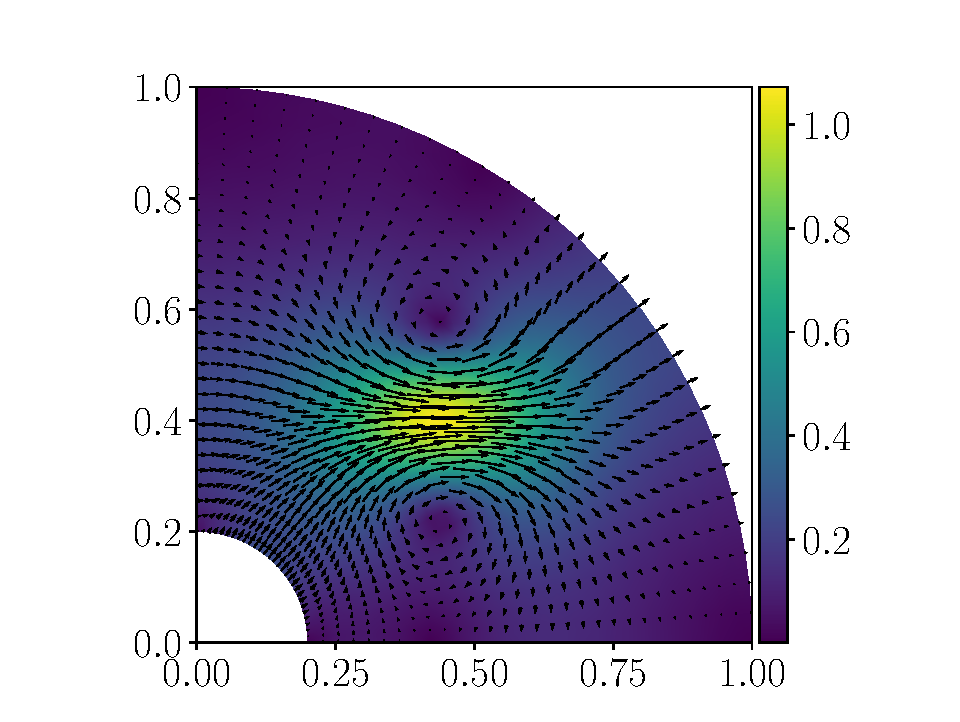
\includegraphics[width=\textwidth]{images/outflow1.pdf}
  \end{subfigure}
  \begin{subfigure}{0.24\textwidth}
    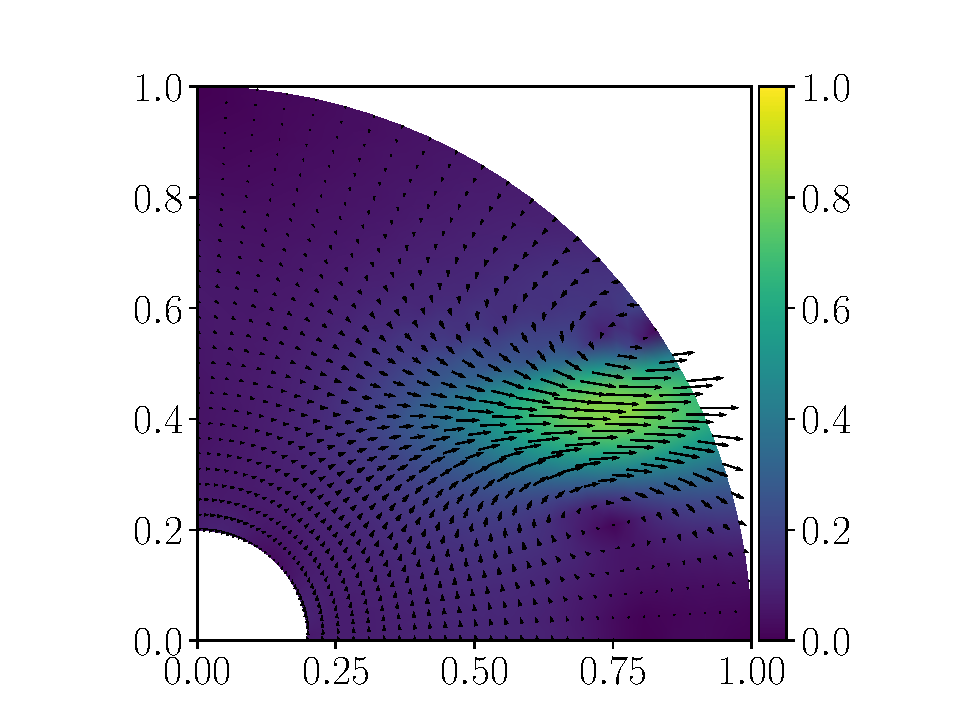
\includegraphics[width=\textwidth]{images/outflow2.pdf}
  \end{subfigure}
  \begin{subfigure}{0.24\textwidth}
    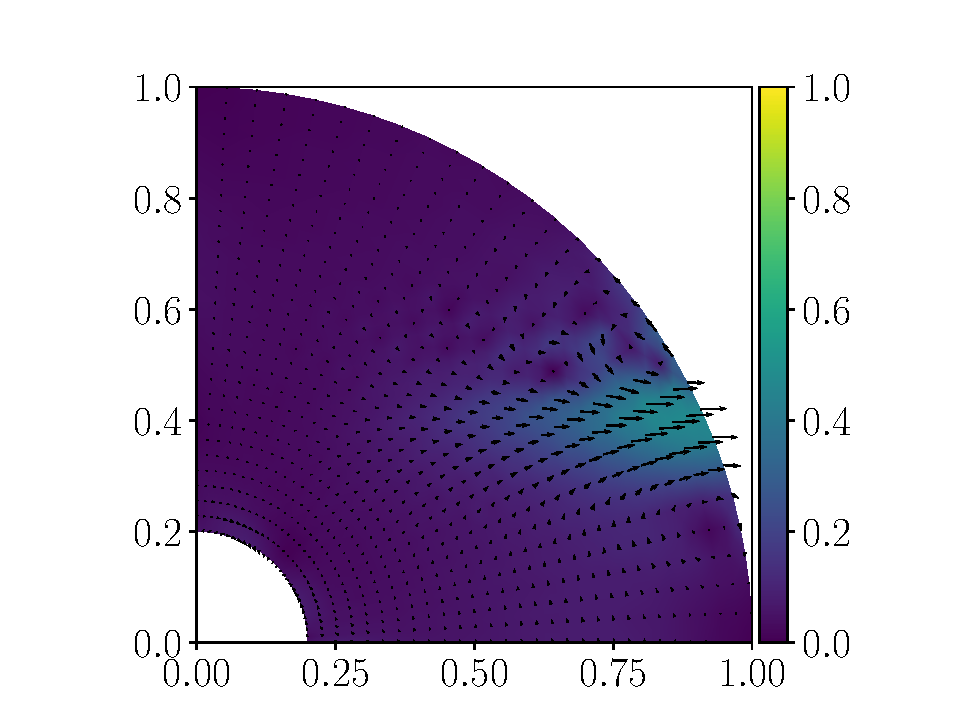
\includegraphics[width=\textwidth]{images/outflow3.pdf}
  \end{subfigure}
  \begin{subfigure}{0.24\textwidth}
    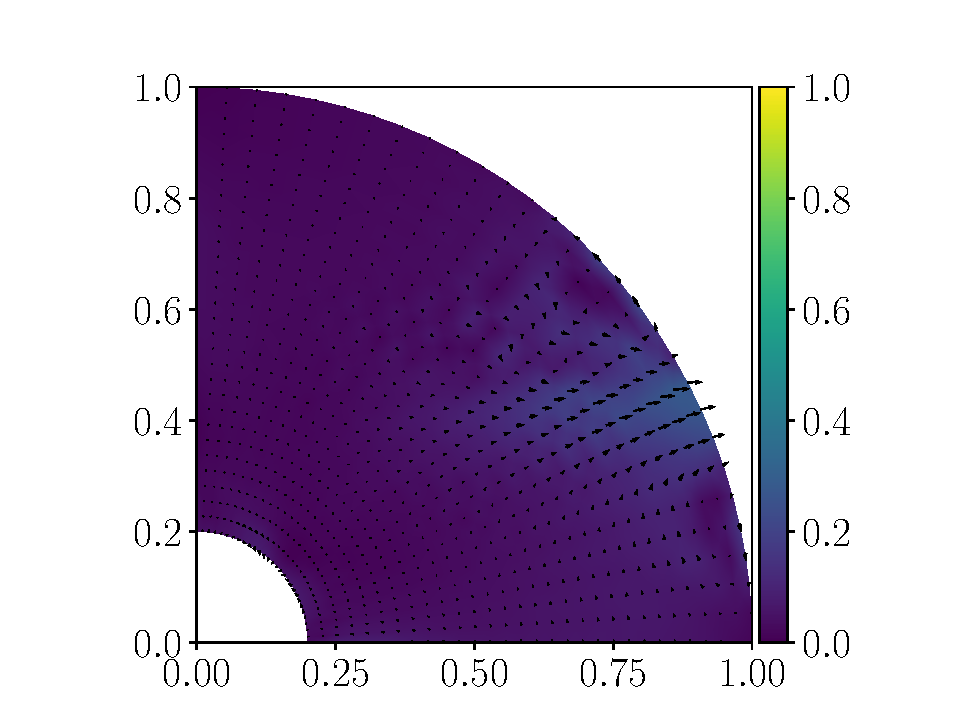
\includegraphics[width=\textwidth]{images/outflow4.pdf}
  \end{subfigure}
  \caption{A simulation initialized with $\vn = \pn = \zeron$, and a Gaussian bell in $\un$, resulting in swirling fluid exiting the domain through a boundary using the stabilized pressure condition.}%
  \label{fig:stab_pressure}
\end{figure}

  \section{Discretization}%
\label{sec:discretization}
Consider a spatial discretization of the incompressible Euler equations~\eqref{eq:euler_nobc_split}.
\begin{subequations}%
\label{eq:discrete_euler_nobc}
  \begin{align}
    \wn_t + \frac{1}{2} \wn \cdotn \nablan \wn + \frac{1}{2} \divn (\wn \wn^\dagger) &= -\nablan \pn \label{eq:discrete_momentum} \\
    \divn \wn &= \zeron \,, \label{eq:discrete_divergence}
  \end{align}
\end{subequations}
where $\wn$ and $\pn$ are time dependent grid functions. The form~\eqref{eq:discrete_euler_nobc} is particularly convenient for discrete energy analysis since the continuous energy analysis can be replicated. Indeed, both Lemma~\ref{lemma:convection2} and Proposition~\ref{prop:energy2} hold discretely (the proofs are identical, simply replace the normal letters by bold letters), resulting in the discrete energy:

\begin{proposition}\label{prop:discrete_energy}
  The semidiscrete incompressible Euler equations~\eqref{eq:discrete_euler_nobc} imply that
  \begin{equation}\label{eq:discrete_boundary_terms}
    \frac{d}{dt} \|\wn\|_{\Omega_h}^2
      = -\ipbnfull{\wnn}{|\wn|^2} - 2\ipbnfull{\wnn}{\pn} + 2\ipn{\pn}{\divn \wn}\,.
  \end{equation}
\end{proposition}
\begin{remark}
  We do not omit the term $2\ipn{\pn}{\divn \wn}$ in Proposition~\ref{prop:discrete_energy} even though it vanishes by~\eqref{eq:discrete_divergence}. This is because it is sometimes useful to make small perturbations to the discrete divergence (i.e.\ allow for local nonzero divergence at a boundary) in order to cancel the pressure term $-2\ipbn{\wnn}{\pn}$ (see the discrete boundary treatment in Section~\ref{sec:discrete_boundary_conditions}).
\end{remark}

For implementation purposes it is better to write~\eqref{eq:discrete_euler_nobc} in more explicit form as
  \begin{equation}
    \label{eq:discrete_euler_explicit}
    \begin{bmatrix}
      \un_t \\
      \vn_t \\
      \zeron
    \end{bmatrix}
    + \euln(\un, \vn, \pn) = \zeron \,,
  \end{equation}
  where
  \begin{equation*}
    \euln(\un, \vn, \pn) =
    \begin{bmatrix}
      \euln_1 & \euln_2 & \euln_3
    \end{bmatrix}^\dagger
  \end{equation*}
  and
  \begin{equation*}
    \begin{aligned}
      \euln_1 &= \frac{1}{2} \un \Dx \un + \frac{1}{2} \Dx \un \un + \frac{1}{2} \vn \Dy \un + \frac{1}{2} \Dy \un \vn + \Dx \pn \\
      \euln_2 &= \frac{1}{2} \vn \Dy \vn + \frac{1}{2} \Dy \vn \vn + \frac{1}{2} \un \Dx \vn + \frac{1}{2} \Dx \un \vn + \Dy \pn \\
      \euln_3 &= \Dx \un + \Dy \vn \,.
    \end{aligned}
  \end{equation*}
\noindent The discretization~\eqref{eq:discrete_euler_explicit} defines a set of differential algebraic equations. These equations are not yet ready to be evolved in time since they do not take into account any boundary conditions. However, the Jacobian of the discrete spatial operator in~\eqref{eq:discrete_euler_nobc} is a key component in any implicit timestepping scheme. The Jacobian can be derived using the following observations. Let $\fn, \gn : \mathbb{R}^n \to \mathbb{R}^n$ be vector-valued differentiable functions and define the diagonal matrices
\[
  \diagn{\fn} =
  \begin{pmatrix}
    f_1 &     &        &     \\
        & f_2 &        &     \\
        &     & \ddots &     \\
        &     &        & f_n \\
  \end{pmatrix}
  \text{ and }
  \diagn{\gn} =
  \begin{pmatrix}
    g_1 &     &        &     \\
        & g_2 &        &     \\
        &     & \ddots &     \\
        &     &        & g_n \\
  \end{pmatrix} \,.
\]
It is readily seen that the Jacobian $J_{\fn\gn}$ of the elementwise product $\fn\gn$ satisfies the following product rule:
\begin{equation}
  \label{eq:jacobian_product_rule}
  J_{\fn\gn} = \diagn{\fn}J_{\gn} + \diagn{\gn}J_{\fn} \,.
\end{equation}
Furthermore, the Jacobian is linear in the sense that for any $n$-by-$n$ matrices $A$ and $B$ we have
\begin{equation}
  \label{eq:jacobian_linear}
  J_{A\fn + B\gn} = AJ_{\fn} + BJ_{\gn} \,.
\end{equation}
Applying these Jacobian properties to $\euln$ yields the following proposition.

\begin{proposition}
  The Jacobian $J_{\euln}$ of the discrete operator $\euln$ in~\eqref{eq:discrete_euler_explicit} is
  \begin{equation*}
    J_{\euln} =
    \begin{pmatrix}
      \nablan_{\un} \euln_1 & \nablan_{\vn} \euln_1 & \nablan_{\pn} \euln_1 \\
      \nablan_{\un} \euln_2 & \nablan_{\vn} \euln_2 & \nablan_{\pn} \euln_2 \\
      \nablan_{\un} \euln_3 & \nablan_{\vn} \euln_3 & \nablan_{\pn} \euln_3
    \end{pmatrix}
  \end{equation*}
  where
  \begin{align*}
    \nablan_{\un} \euln_1 &= \frac{1}{2} \left(\diagn{\un}\Dx + \diagn{\Dx\un} + 2\Dx\diagn{\un} + \diagn{\vn}\Dy + \Dy\diagn{\vn}\right) \\
    \nablan_{\vn} \euln_1 &= \frac{1}{2} \left(\diagn{\Dy\un} + \Dy\diagn{\un}\right) \\
    \nablan_{\pn} \euln_1 &= \Dx \\
    \nablan_{\un} \euln_2 &= \frac{1}{2} \left(\diagn{\Dx\vn} + \Dx\diagn{\vn}\right) \\
    \nablan_{\vn} \euln_2 &= \frac{1}{2} \left(\diagn{\vn}\Dy + \diagn{\Dy\vn} + 2\Dy\diagn{\vn} + \diagn{\un}\Dx + \Dx\diagn{\un}\right) \\
    \nablan_{\pn} \euln_2 &= \Dy \\
    \nablan_{\un} \euln_3 &= \Dx \\
    \nablan_{\vn} \euln_3 &= \Dy \\
    \nablan_{\pn} \euln_3 &= \zeron \,.
  \end{align*}
\end{proposition}

\begin{proof}
  Let us find the first couple of terms in $\nablan_{\un} \euln_1$. The proofs for the other blocks are similar. Consider the first term $\frac{1}{2}\un \Dx \un$ of $\euln_1$. Let $\fn = \un$ and $\gn = \Dx \un$. Then $J_{\fn} = \In$ and $J_{\gn} = \Dx$. Hence, by~\eqref{eq:jacobian_product_rule},
  \begin{equation*}
    \nablan_{\un} \left( \frac{1}{2}\un \Dx \un \right) = \frac{1}{2} (\diagn{\un}\Dx + \diagn{\Dx \un}) \,.
  \end{equation*}
  Similarly, for the second term $\frac{1}{2} \Dx \un \un$ of $\euln_1$, we set $\fn = \un$ and $\gn = \un$. Then $J_{\fn} = J_{\gn} = \In$ and by~\eqref{eq:jacobian_product_rule} and~\eqref{eq:jacobian_linear} we get
  \begin{equation*}
    \nablan_{\un} \left( \frac{1}{2} \Dx \un \un \right) = \Dx \diagn{\un} \,.
  \end{equation*}

\end{proof}

  \section{Discrete boundary conditions}%
\label{sec:discrete_boundary_conditions}
In this section we describe how to implement the boundary conditions from Section~\ref{sec:boundary_conditions} using penalty terms. The main idea is to associate to each boundary a penalty operator $\satn(\un, \vn, \pn)$ which is added to the Euler spatial operator $\euln(\un, \vn, \pn)$. Similarly, the Jacobian of $\satn$ is added to the Jacobian of $\euln$, since $J_{\euln+\satn} = J_{\euln} + J_{\satn}$.

For a given boundary condition $H(u,v,p) = g$, a penalty operator $\satn$ will typically have the form
$
  \satn =
  \begin{bmatrix}
    \satn_1 & \satn_2 & \satn_3
  \end{bmatrix}^\dagger
$,
where
$
  \satn_i = C_i (H(\un, \vn, \pn) - \gn)
$,
and $C_i$ is a penalty coefficient. When a boundary condition is not satisfied, its penalty operator $\satn$ will add appropriate contributions to $\euln$, pushing the solution toward compliance with the boundary condition. A penalty operator is ideally built such that it cancels the growth terms in~\eqref{eq:discrete_boundary_terms}, or replaces them with data, so we know that the kinetic energy cannot grow uncontrollably.

\begin{definition}\label{def:stable_penalty}
  A penalty operator
  $
    \satn^d =
    \begin{bmatrix}
      \satn^d_1 & \satn^d_2 & \satn^d_3
    \end{bmatrix}^\dagger
  $
  for the boundary $\Gamma_d$ is called \emph{stable} if
  \begin{equation*}
    \text{PT} + \text{BT} \geq g_d \,,
  \end{equation*}
  where
  \begin{equation*}
    \text{PT} = 2\ipn{\un}{\satn^d_1} + 2\ipn{\vn}{\satn^d_2} + \ipn{\pn}{\satn^d_3} \,,
  \end{equation*}
  \begin{equation*}
    \text{BT} = \ipbn{\wnn}{|\wn|^2} + 2\ipbn{\wnn}{\pn} \,,
  \end{equation*}
  and $g_d$ is a bounded time dependent function. Furthermore, if $\text{PT} + \text{BT} = 0$, then $\satn^d$ is called \emph{conservative}. Finally, if $\text{PT} + \text{BT} > 0$, then $\satn^d$ is called \emph{dissipative}.
\end{definition}

\begin{remark}
  Note that any conservative or dissipative penalty operator is also stable.
\end{remark}

Definition~\ref{def:stable_penalty} is motivated by the following proposition, ensuring that the discretization~\eqref{eq:discrete_euler_explicit}, combined with stable penalty operators, is stable with respect to the kinetic energy.

\begin{proposition}
  Assume that for each boundary $\Gamma_d$ we have a stable penalty operator $\satn^d$. If $\un, \vn, \pn$ solves the system
  \begin{equation*}
    \begin{bmatrix}
      \un_t \\
      \vn_t \\
      \zeron
    \end{bmatrix}
    + \euln + \sum_d \satn^d = \zeron \,,
  \end{equation*}
  then
  \begin{equation*}
    \frac{d}{dt} \normn{\wn}^2 \leq g \,,
  \end{equation*}
  where $g$ is a bounded time dependent function.
\end{proposition}

\begin{proof}
 By using Proposition~\ref{prop:discrete_energy}, and adding the contribution from the penalty terms, we get that
\begin{equation}
\begin{aligned}
   \frac{d}{dt} \|\wn\|_{\Omega_h}^2
   = & - \sum_d\ipbn{\wnn}{|\wn|^2 + 2p} \\
    & - 2 \sum_d
    \left( \ipn{\un}{\satn_1^d} + \ipn{\vn}{\satn_2^d} + \ipn{\pn}{\satn_3^d}\right)
    \\
    =& - \sum_d BT + PT \le \sum_d g_d
    \,.
\end{aligned}
\label{eq:discrete_boundary_proof}
\end{equation}
In~\eqref{eq:discrete_boundary_proof}, the term $\div \wn$ has been replaced by $- \sum_d\satn^d_3$. The last inequality holds since the penalty operator is stable.
\end{proof}

Let us start by introducing the concept of a discrete lifting operator $\Lng = \Pn^{-1} \Png$ associated to the boundary $\Gamma_d$. The lifting operator $\Lng$ is a sparse diagonal matrix with nonzero entries in the positions corresponding to the boundary $\Gamma_d$, which has the property that
\begin{equation}
  \ipn{\un}{\Lng \phin} = \ipbn{\un}{\phin} \,.
\end{equation}
Lifting operators are used in all our penalty terms because they allow us to convert integrals over $\Omega_h$ to integrals over $\Gamma_d$ in the energy analysis.

Below we list Penalty Operator/Jacobian pairs $(\satn,J_{\satn})$ for the boundary conditions described in Section~\ref{sec:boundary_conditions}, on the form
  \begin{equation*}
    \satn =
    \begin{bmatrix}
      \satn_1 & \satn_2 & \satn_3
    \end{bmatrix}^\dagger \,, \quad
    J_{\satn} =
    \begin{pmatrix}
      \nablan_{\un} \satn_1 & \nablan_{\vn} \satn_1 & \nablan_{\pn} \satn_1 \\
      \nablan_{\un} \satn_2 & \nablan_{\vn} \satn_2 & \nablan_{\pn} \satn_2 \\
      \nablan_{\un} \satn_3 & \nablan_{\vn} \satn_3 & \nablan_{\pn} \satn_3
    \end{pmatrix} \,.
  \end{equation*}
NOTE:\@ For the penalty operators considered in this paper, all blocks in $J_{\satn}$ are diagonal $N_x N_y$-by-$N_x N_y$ matrices. We shall therefore allow ourselves to omit the underline-notation and let it be understood that column vectors represent diagonal matrices in this context.

\subsection{Solid wall}%
\label{sub:solid_wall_discrete}
\subsubsection*{Penalty operator}
$\satn_1 = -\frac{1}{2} \Lng \un \wnn,\,$
$\satn_2 = -\frac{1}{2} \Lng \vn \wnn,\,$
and
$\satn_3 = -\Lng \wnn$.

\subsubsection*{Jacobian}
$
  \nablan_{\pn} \satn_1 =
  \nablan_{\pn} \satn_2 =
  \nablan_{\pn} \satn_3 = \zeron
$
and
\begin{align*}
  \nablan_{\un} \satn_1 = -\frac{1}{2} \Lng (\un\nnx + \wnn) \,, \quad
  \nablan_{\un} \satn_2 = -\frac{1}{2} \Lng \vn\nnx \,, \quad
  \nablan_{\un} \satn_3 = -\Lng \nnx \,, \\
  %
  \nablan_{\vn} \satn_1 = -\frac{1}{2} \Lng \un \nny \,, \quad
  \nablan_{\vn} \satn_2 = -\frac{1}{2} \Lng (\vn\nny + \wnn) \,, \quad
  \nablan_{\vn} \satn_3 = -\Lng \nny \,.
\end{align*}
\subsubsection*{Stability}
We have $\ipn{2\un}{\satn_1} = -\ipbn{\un^2}{\wnn}, \, \ipn{2\vn}{\satn_2} = -\ipbn{\vn^2}{\wnn}$, and $\ipn{\pn}{\satn_3} = -\ipbn{\pn}{\wnn}$. Hence $\satn$ is conservative by Definition~\ref{def:stable_penalty}.
\subsection{Pressure outflow}%
\label{sub:pressure_outflow}
\subsubsection*{Penalty operator}
$\satn_1 = -\Lng \nnx \pn,\,$
$\satn_2 = -\Lng \nny \pn,\,$
and
$\satn_3 = \zeron$.

\subsubsection*{Jacobian}
  $\nablan_{\pn} \satn_1 = -\Lng \nnx,\,$
  $\nablan_{\pn} \satn_2 = -\Lng \nny,\,$
  and the rest are $\zeron$.

\subsubsection*{Stability}
We have $\ipn{2\un}{\satn_1} = -\ipbn{2\un \nnx}{\pn}, \, \ipn{2\vn}{\satn_2} = -\ipbn{2\vn \nny}{\pn}$, and $\ipn{\pn}{\satn_3} = 0$. Hence, if $\wnn \geq \zeron$, then $\satn$ is dissipative by Definition~\ref{def:stable_penalty}.


\subsection{Stabilized pressure outflow}%
\label{sub:stabilized_pressure_outflow}
Note: For this boundary operator to be differentiable we approximate the Heaviside function $h$ in Section~\ref{sub:stab_pressure} by a sigmoid function $h(\wcn) = 1/(e^{\wcn} + 1)$.
\subsubsection*{Penalty operator}
  \begin{equation*}
    \begin{aligned}
      \satn_1 &= -\Lng \nnx \left(h(\wnn)|\wn|^2 + \pn\right) \,, \\
      \satn_2 &= -\Lng \nny \left(h(\wnn)|\wn|^2 + \pn\right) \,, \\
      \satn_3 &= \zeron\,.
    \end{aligned}
  \end{equation*}

\subsubsection*{Jacobian}
\begin{align*}
  \nablan_{\un} \satn_1 &= -\Lng \nnx\left(\nablan_{u}h(\wnn)|\wn|^2 + 2h(\wnn) (\wnn \nnx - \wtn \nny)\right) \\
\nablan_{\vn} \satn_1 &= -\Lng \nnx\left(\nablan_{v}h(\wnn)|\wn|^2 + 2h(\wnn) (\wnn \nny + \wtn \nnx)\right) \\
  \nablan_{\pn} \satn_1 &= -\Lng \nnx \\
  \nablan_{\un} \satn_2 &= -\Lng \nny\left(\nablan_{u}h(\wnn)|\wn|^2 + 2h(\wnn) (\wnn \nnx - \wtn \nny)\right) \\
  \nablan_{\vn} \satn_2 &= -\Lng \nny\left(\nablan_{v}h(\wnn)|\wn|^2 + 2h(\wnn) (\wnn \nny + \wtn \nnx)\right) \\
  \nablan_{\pn} \satn_2 &= -\Lng \nny
\end{align*}
where
\begin{align*}
  \nablan_{\un}h(\wnn) &= -\frac{e^{\wnn}}{{(e^{\wnn} + 1)}^2}\nnx \,,
  \\
  \nablan_{\vn}h(\wnn) &= -\frac{e^{\wnn}}{{(e^{\wnn} + 1)}^2}\nny \,.
\end{align*}
Furthermore,
\[ \nablan_{\un} \satn_3 = \nablan_{\vn} \satn_3 = \nablan_{\pn} \satn_3 = \zeron \,. \]

\subsubsection*{Stability}
We have
\begin{align*}
  \ipn{2\un}{\satn_1} & = -\ipbn{2\un \nnx}{h(\wnn)|\wn|^2 + \pn} \\
  \ipn{2\vn}{\satn_2} & = -\ipbn{2\vn \nny}{h(\wnn)|\wn|^2 + \pn} \\
  \ipn{\pn}{\satn_3}  & = 0 \,.
\end{align*}
Hence $\satn$ is conservative if $\wnn \leq 0$ and dissipative otherwise.

\subsection{Inflow}%
\label{sub:inflow}
\subsubsection*{Penalty operator}
  \begin{equation*}
    \begin{aligned}
      \satn_1 &= -\Lng \nnx \wnn (\wnn - \gn_n) + \Lng \nny \wnn (\wtn - \gn_s)\,, \\
      \satn_2 &= -\Lng \nny \wnn (\wnn - \gn_n) - \Lng \nnx \wnn (\wtn - \gn_s)\,, \\
      \satn_3 &= -\Lng(\wnn - \gn_n).
    \end{aligned}
  \end{equation*}

\subsubsection*{Jacobian}
  \begin{equation*}
    \begin{aligned}
      \nablan_{\un} \satn_1 &= -\Lng \left(\nnx^2(2\wnn - \gn_n) + \nny^2\wnn + \nnx \nny (\wtn - \gn_t)\right)\,, \\
      \nablan_{\vn} \satn_1 &= \phantom{-}\Lng \left(\nny^2(\wtn - \gn_t) - \nnx\nny(\wnn - \gn_n)\right)\,, \\
      \nablan_{\un} \satn_2 &= -\Lng \left(\nnx^2(\wtn - \gn_t) + \nnx\nny(\wnn - \gn_n)\right)\,, \\
      \nablan_{\vn} \satn_2 &= -\Lng \left(\nny^2(2\wnn - \gn_n) + \nnx^2\wnn + \nnx \nny (\wtn - \gn_t)\right) \,, \\
      \nablan_{\un} \satn_3 &= -\Lng \nnx \,, \\
      \nablan_{\vn} \satn_3 &= -\Lng \nny \,,
    \end{aligned}
  \end{equation*}
  and the rest are $\zeron$.

\subsubsection*{Stability}
As seen in Section~\ref{sub:inflow}, imposing Dirichlet conditions at an inflow boundary do not result in a bound. We get 
\begin{align*}
  PT + BT & = 
  %\ipn{2\un}{\satn_1}  + \ipn{2\vn}{\satn_2} + \ipn{\pn}{\satn_3} 
  %+ \ipbn{\wnn}{|\wn|^2} + 2\ipbn{\wnn}{\pn}
  %\\
  %& = -\ipbn{2\wnn^2}{\wnn-\gn_n} -\ipbn{2\wnn \wtn}{\wtn-\gn_s} 
  %- \ipbn{2\pn}{\wnn-\gn_n}
  %\\
  %& +\ipbn{\wnn}{|\wn|^2} + 2\ipbn{\wnn}{\pn}
  %\\
  %& = 
  \ipbn{\wnn}{-\wnn^2 + 2 \wnn \gn_n} + \ipbn{\wnn}{-\wtn^2 + 2 \wtn \gn_n}
\end{align*}

  \section{The fully discrete scheme}%
\label{sec:fully_discrete}
To evolve the system \eqref{eq:ins_semi_discrete} in time, we will for simplicity and ease of explanation use the implicit Backward Euler method. More accurate and efficient methods could be used in the same manner in practice.  For an ordinary differential system of equations of the form
\begin{equation*}
 \Mn \soln_t + \Hn(\soln) = 0
 \, ,
\end{equation*}
where $\soln$ is a function defined on the grid and $\Mn$ is a constant matrix, the backward Euler schemes becomes 
\begin{equation}
  \frac{\Mn (\soln^{i+1} - \soln^i)}{\Delta t} + \Hn(\soln^{i+1}) = 0
  \,.
  \label{eq:backward_euler}
\end{equation}
In~\eqref{eq:backward_euler}, $\Delta t$ is the size of the time step and the superindices $i$ and $i+1$ are the solution at time level $i$ and $i+1$, respectively.

In order to obtain $\soln^{i+1}$, the system of nonlinear equations in~\eqref{eq:backward_euler} must be solved. One strategy is to first form the function in \eqref{eq:intro}, which results in
\begin{equation}
  \Fn(\soln^{i+1}) = 
  \frac{\Mn (\soln^{i+1} - \soln^i)}{\Delta t} + \Hn(\soln^{i+1})
  \,.
  \label{eq:F_function}
\end{equation}
If we find a vector $\soln^*$ such that $\Fn(\soln^*) = 0$, then $\soln^{i+1} = \soln^*$. To solve~\eqref{eq:F_function}, we employ Newton's method~\cite{quarteroni2010numerical}, which is described in \cref{alg:newton}. This allows us to solve a sequence of linear systems of equations and arrive at an approximation of $\soln^{i+1}$.
\begin{algorithm}
\caption{Newton's method}
\label{alg:newton}
\begin{algorithmic}
\STATE{\ \  Input: $\soln^0$ and tolerance $tol$}
\STATE{Output: An approximation of $\soln^*$, where $\Fn(\soln^*) = 0$}
\FOR{$j = 0,1,2, \dots$}
\STATE{solve $J_{\Fn}(\soln^j)\bm{h}^j   = - \Fn(\soln^j)$ \\
set   $\soln^{j+1}  = \soln^j + \bm{h}^j$ \\
\IF{$\|\Fn(\soln^{j+1})\| < tol$} 
		\RETURN  $\soln^{j+1}$
	     \ENDIF}
\ENDFOR
\end{algorithmic}
\end{algorithm}

For the INS equations, $\soln = \wn$, $\Hn(\soln) = \euln(\soln) - \satn(\soln)$, and $\Mn = \Itn$. Hence,~\eqref{eq:F_function} becomes
\begin{equation}
  \Fn(\wn^{i+1}) = 
  \frac{1}{\Delta t} 
  \left(
    \begin{bmatrix}
      \un^{i+1} \\ \vn^{i+1} \\ \zeron
    \end{bmatrix}
    -
    \begin{bmatrix}
      \un^{i} \\ \vn^{i} \\ \zeron
    \end{bmatrix}
    \right)
    + \euln(\wn^{i+1}) - \satn(\wn^{i+1})
  \, . 
  \label{eq:F_function_euler}
\end{equation}
Furthermore, $J_{\Hn}(\wn) = J_{\euln}(\wn) - J_{\satn}(\wn)$, which yields
\begin{equation}
  J_{\Fn}(\wn) =  
  \frac{1}{\Delta t}
  \Itn
  +
  J_{\euln}(\wn)
  -
  J_{\satn}(\wn)
  \, ,
  \label{eq:backward_euler_jacobian}
\end{equation} 
to be used in the Newton iterations. In \eqref{eq:backward_euler_jacobian}, $J_{\euln}(\wn)$ and $J_{\satn}(\wn)$ are given in \Cref{prop:ins} and \Cref{prop:sat}, respectively.

\section{Numerical Experiments}
\label{sec:numerical_experiments}
A simple finite-difference approximation of the Jacobian is given by \cite{knoll2004jacobian} 
\begin{equation}
  J_{i,j} \approx \hat{J}_{i,j} = \frac{\Fn_i(\wn + \delta_j \en_j) - \Fn_i(\wn)}{\delta_j}
  \, .
  \label{eq:J_approx}
\end{equation}
The approximation in \eqref{eq:J_approx} was used during the implementation of the analytical expression of $J_{\Fn}$ since we expected $\|J - \hat{J}\|_{\infty}$ to be small. This allowed us to write unit tests ensuring that the Jacobian has been correctly implemented, by comparing it to the approximation. In \eqref{eq:J_approx}, a small $\delta$ leads to a good approximation. However, note that if $\delta$ is chosen too small, the approximation will be contaminated by floating-point roundoff errors, which limits the practically achievable accuracy of $J$ \cite{knoll2004jacobian}.

Computing difference approximations of the Jacobian also allowed us to compare the efficiency of Newton's method using approximate versus analytical Jacobians. Note that computing the approximation \eqref{eq:J_approx} requires $n$ evaluations of $\Fn$, resulting in $O(n^2)$ complexity, compared to the $O(n)$ complexity of evaluating the exact Jacobian. \Cref{tab:efficiency} shows the execution times for evaluating the analytical Jacobian versus computing the approximation~\eqref{eq:J_approx} at increasing resolutions.

\begin{table}[ht]
  \centering
  \begin{tabular}{|c|c|c|}
    \hline
    Resolution & Exact & FD approximation \\
    \hline
    $5 \times 5$ & 0.005s & 0.858s \\
    $10 \times 10$ & 0.006s & 13.85s \\
    $15 \times 15$ & 0.006s & 76.49s \\
    $20 \times 20$ & 0.007s & 261.6s \\
    \hline
  \end{tabular}
  \caption{Execution times for computing the exact Jacobian of $\Fn$ versus the finite difference approximation~\eqref{eq:J_approx}. Even at low resolutions, using difference approximations of the Jacobian is clearly unrealistic.}
  \label{tab:efficiency}
\end{table}

As expected, due to the large number of evaluations of $\Fn$ needed to compute the approximation, such a strategy quickly becomes infeasible.

It is readily seen that the number of floating point operations needed to evaluate the discrete spatial operator $\euln$ grows linearly with the degrees of freedom $n$. Consider for example the term $\An(I_3 \otimes \Dx)\wn$. The first product, $(I_3 \otimes \Dx) \wn$, are finite difference approximations at each point in the grid, resulting in $Cn$ operations, where $C$ depends on the width of the difference stencil. The matrix $\An$ is a $3$-by-$3$ block matrix with diagonal blocks, and so results in another $O(n)$ number of operations. Analogously, the remaning terms in $\euln$ each contribute $O(n)$ operations. The arithmetic complexity of evaluating a penalty term $\satn$ is $O(\sqrt{n})$ (assuming equal resolution in the horizontal and vertical directions), since $\satn$ acts only on the grid boundary. Hence, the arithmetic complexity of evaluating $\Fn$ is $O(n)$.

Let us study the arithmetic complexity of evaluating the Jacobian $J_{\Fn}$ of $\Fn$. Inspecting the form of the Jacobian $J_{\euln}$ in \Cref{prop:ins} we see a number of terms that need to be evaluated. The partial derivatives $\underline{\Dx \un}$, $\underline{\Dy \vn}$, etc, have already been computed as part of the evaluation of $\euln$, and hence can be disregarded. Similarly, terms that do not depend on the solution, such as $\Dx$, $\Dx^2$, etc, can be disregarded since they remain constant throughout the simulation. Finally we have terms of the type $\Un \Dx$, $\Dy \Vn$, etc. These are all products of a diagonal matrix and a banded difference stencil matrix, and each contribute with $O(n)$ operations. Summing the terms uses $O(n)$ operations. Therefore, the arithmetic complexity of evaluating $J_{\euln}$ is $O(n)$. In fact, the number of operations needed to evaluate products like $\Un \Dx$ or $\Dy \Vn$ do not exceed the number of operations needed to compute the discrete partial derivatives involved in $\euln$. Hence, the cost ratio of evaluating $J_{\euln}$ and evaluating $\euln$ is less than $1$ (i.e. the additional cost of evaluating $J_{\euln}$ is small). As before, the arithmetic complexity of evaluating the Jacobian with respect to a boundary penalty $\satn$ is $O(\sqrt{n})$ since it acts only on the boundary of the grid. Thus, the total arithmetic complexity of evaluating $J_{\Fn}$ is less than the cost of evaluating $\Fn$.


\subsection{The order of accuracy}
The method of manufactured solution \cite{roache2002code} is used to verify the implementation. In all computations in this subsection, the initial guess is the solution from the previous time step and the tolerance $tol$ in \Cref{alg:newton} is set to $10^{-12}$.
For the SBP-operators SBP21 and SBP42, the expected orders of accuracy for the system \eqref{eq:ins_semi_discrete} are 2 and 3, respectively~\cite{svard2006order,svard2019convergence}. The manufactured solution we have used is
\begin{equation}
  \begin{aligned}
    u & = 1 + 0.1 \sin(3\pi x-0.01t)\sin(3\pi y-0.01t)
    \\
    v & = \sin(3\pi x-0.01t)\sin(3\pi y-0.01t)
    \\
    p & = \cos(3\pi x-0.01t)\cos(3\pi y-0.01t)
    \, .
 \end{aligned}
 \label{eq:mms_solution}
\end{equation}
Inserting \eqref{eq:mms_solution} into \eqref{eq:ins_continuous} leads to a non-zero right-hand side $\vecs{k}(t,x,y)$, which is evaluated on the grid and added to the right-hand side of \eqref{eq:ins_semi_discrete} by the vector $\vecs{\kn}(t)$. Since $\vecs{\kn}$ is independent of $\wn$, it does not affect the Jacobian. The initial and boundary data are also taken from \eqref{eq:mms_solution}.
The step size is chosen to be $\Delta t = 10^{-5}$ and the computations are terminated at $t = 1$. Next, we compute the pointwise error vector $\vecs{\en}$ and its $L_2$-norm $\|\vecs{\en}\|_{I_3\otimes \Pn}$. The spatial convergence rate for the SBP operators is given by $r = \log(\|\en\|_{i}/\|\en\|_{j})/\log((j-1)/(i-1))$, where $i$ and $j$ refer to the number of grid points in both spatial dimensions. The order of accuracy in space are presented in \cref{tab:convergence_table} and agree well with theory.
\begin{table}
\centering
\setlength{\tabcolsep}{12pt}
\begin{tabular}{c| cc | cc cc}
 \hline
 \hline
 operator
 & \multicolumn{2}{c|}{SBP21}
 & \multicolumn{2}{c}{SBP42}
 \\
\hline
 \hline
N & $\|\en\|$ & $r$ &$\|\en\|$ & $r$
\\
\hline
21 & 4.13e-02 & --   & 1.90e-02 & -- 
\\   
41 & 9.73e-03 & 2.16 & 2.19e-03 & 3.23
\\
61 & 4.17e-03 & 2.13 & 6.34e-04 & 3.12  
\\
81 & 2.28e-03 & 2.12 & 2.70e-04 & 3.01
\\
\hline
Theoretical && 2 && 3
\end{tabular}
\caption{Error and convergence rate.}%
\label{tab:convergence_table}
\end{table}

Next, we consider the steady-state problem of \eqref{eq:ins_continuous} and \eqref{eq:ins_semi_discrete}, which means that the goal is to find $\wn^*$ such that
\begin{equation}
   \euln(\wn^*) = \satn(\wn^*)
   \, .
   \label{eq:ins_steady_state}
\end{equation}
As before, we want to find an approximation to the vector $\wn^*$ which satisfies
\begin{equation}
  \Fn (\wn^*) = \euln(\wn^*) - \satn(\wn^*) = 0  
  \, .
  \label{eq:F_steady_state}
\end{equation}
The Jacobian of $\Fn$ is $J_{\Fn}(\wn) = J_{\euln}(\wn) - J_{\satn}(\wn)$. 
When the iterate $\wn^k$ is far away from $\wn^*$, Newton's method may not converge and other techniques must initially be applied. We choose the SOR method \cite{quarteroni2010numerical} 
until $\|F(\wn^k)\|_\infty$ is sufficiently small. For SOR, the next iterate is given by $\wn^{k+1} = \wn^k(1-\alpha) + (\wn^k - \hn^k)\alpha$, where $\hn^k$ is the Newton step from \Cref{alg:newton} and $\alpha \in (0,1]$.

To verify our procedure, we choose the steady manufactured solution to be \cite{kovasznay1948laminar} 
\begin{equation}
  \begin{aligned}
    u & = 1-e^{\lambda x} \cos(2\pi y)
    & v & = \frac{1}{2 \pi}\lambda e^{\lambda x}\sin(2\pi y)
    \\
    p & = \frac{1}{2}\left(1 - e^{2\lambda x}\right)
    & \lambda & = \frac{1}{2 \epsilon} - \sqrt{\frac{1}{4 \epsilon^2} + 4 \pi^2}
 \end{aligned}
 \label{eq:mms_solution_steady}
\end{equation}
and the computational domain is changed to $\Omega = [-0.5,1]\times [-1,1]$ for $\epsilon = 1/20$. Inserting \eqref{eq:mms_solution_steady} into the time-independent version of \eqref{eq:ins_continuous} leads to $\vecs{k}(t,x,y) = 0$. The initial guess is $\wn^0 = (1,1, \dots, 1)^\top$ and the tolerance $tol$ in \Cref{alg:newton} is again set to $10^{-12}$. 
%We used $\alpha = 0.5$ until $\|F(\soln^k)\|_\infty < 10^3$. 
\Cref{tab:convergence_table_steady} shows the error and convergence rates, which again agrees well with theory. In \Cref{fig:streamlines}, the streamlines and the velocity field is illustrated for the converged solution on the grid containing $100\times 100$ points. They agree well with previous results \cite{kovasznay1948laminar}. 

\subsection{The convergence rate of the Newton iteration}
Next, we will test the main development in this paper. For $\wn^k$ sufficiently close to $\wn^*$, Newton's method converges quadratically in any norm \cite{quarteroni2010numerical}, which means that $e_{k+1} = C e_k^2$, where $C$ varies marginally between iterations and $e_k = \|\wn^k - \wn^*\|$. To verify that, we consider a grid of size $100\times 100$ with the SBP42 operator. The exact solution $\wn^*$ is approximated by the last iterate. By the assumption that $C$ is constant, the relation

\[
  \frac{e_{k+1}}{e_{k}} \approx
  \left(\frac{e_{k}}{e_{k-1}}\right)^p
\]
is obtained for a general convergence rate $p$, which yields
\[
   p \approx \frac{\log(e_{k+1}/e_k)}{\log(e_{k}/e_{k-1})}
   \, .
\]
The error $e_k = \|\wn^k-\wn^*\|_\infty$ is presented in \Cref{tab:newton_convergence} together with the estimations of $p$. The convergence rate agrees well with the expected theoretical one, which verifies that the Jacobian of $\Fn$ is correct. 
\begin{table}
\centering
\setlength{\tabcolsep}{12pt}
\begin{tabular}{c| cc | cc cc}
 \hline
 \hline
 operator
 & \multicolumn{2}{c|}{SBP21}
 & \multicolumn{2}{c}{SBP42}
 \\
\hline
 \hline
N & $\|\en\|$ & $r$ &$\|\en\|$ & $r$
\\
\hline
21 & 2.04e-01 & --   & 4.95e-02 & --  \\
41 & 4.56e-02 & 2.16 & 6.86e-03 & 2.85 \\
61 & 2.04e-02 & 1.98 & 2.20e-03 & 2.80 \\
81 & 1.16e-02 & 1.97 & 9.76e-04 & 2.83 \\
101& 7.46e-03 & 1.97 & 5.16e-04 & 2.85    
\\
\hline
Theoretical && 2 && 3
\end{tabular}
\caption{Error and (accuracy) convergence rate of \eqref{eq:mms_solution_steady}.}%
\label{tab:convergence_table_steady}
\end{table}

\begin{figure}
 \centering
  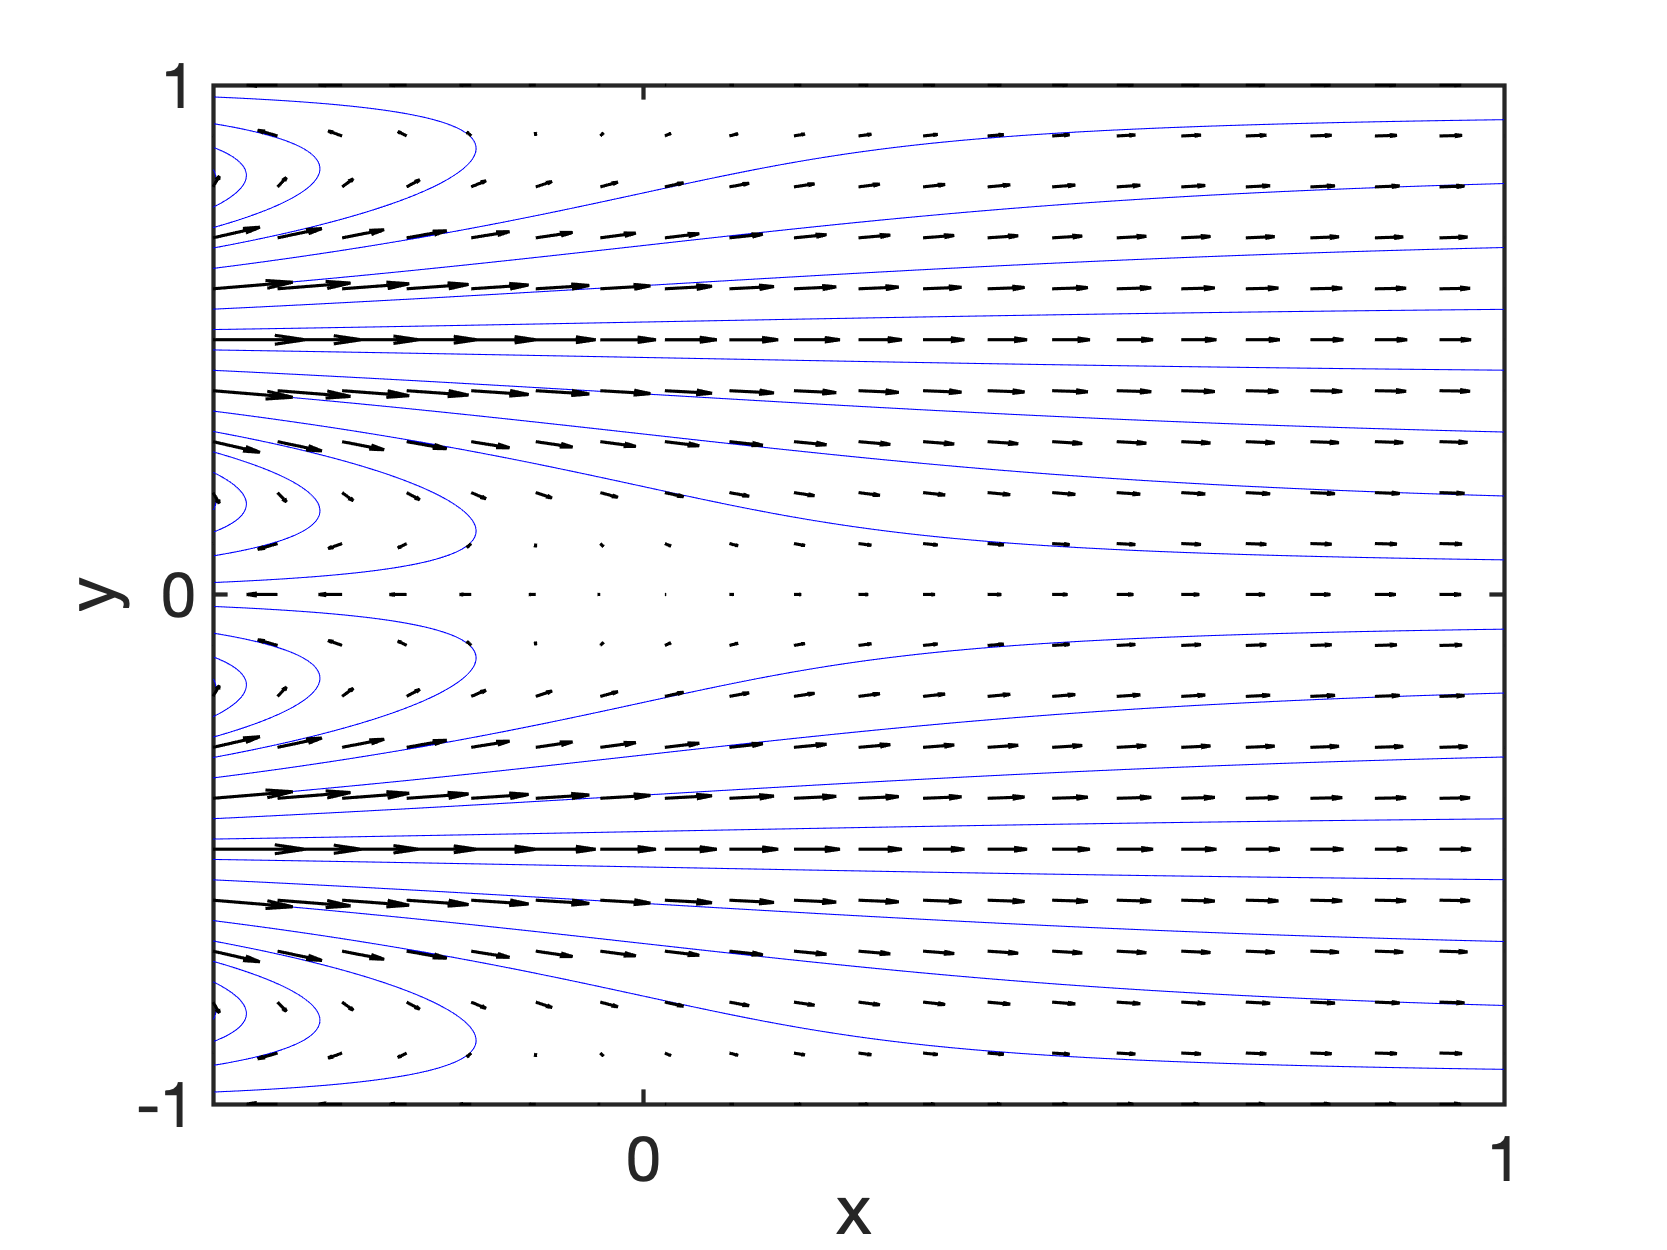
\includegraphics[scale = 0.3]{images/kovaszany}
  \caption{Streamlines and the velocity field of \eqref{eq:mms_solution_steady}.}
  \label{fig:streamlines}
\end{figure}
\begin{table}
\centering
\caption{Errors and the estimated (iterative) convergence rates of \eqref{eq:mms_solution_steady}.}
\begin{tabular}{c| cc }
 \hline
k & $\|e_k\|_\infty$ & $p$
\\
\hline
1 & 3.56e+00  & -- \\
2 & 1.85e+01  & --  \\
3 & 1.89e+00  & -1.38 \\
4 & 1.21e+00  &  0.20 \\
5 & 5.53e-01  &  1.74 \\
6 & 1.10e-01  &  2.07 \\
7 & 3.21e-03  &  2.19 \\
8 & 3.31e-06  &  1.94 \\
9 & 4.14e-12  &  1.98 \\
\hline
Theoretical && 2
\end{tabular}
\label{tab:newton_convergence}
\end{table}

Next, we move on to a more realistic case where the boundary data is set to $g_1 = 1$, $g_2 = g_3 = g_4 = g_5 = g_6 = 0$ and $\epsilon = 0.01$, which will lead to a boundary layer. The computations are performed on $\Omega = [0,1]^2$ with $200\times 200$ grid points with the SBP42 operator. \Cref{fig:boundary_layer} illustrates $\un$ for the converged solution and the iterative convergence order, $p$, is presented in \Cref{tab:boundary_layer}. The estimated iterative convergence order agrees well with what is theoretically expected. 

\begin{figure}
  \centering
  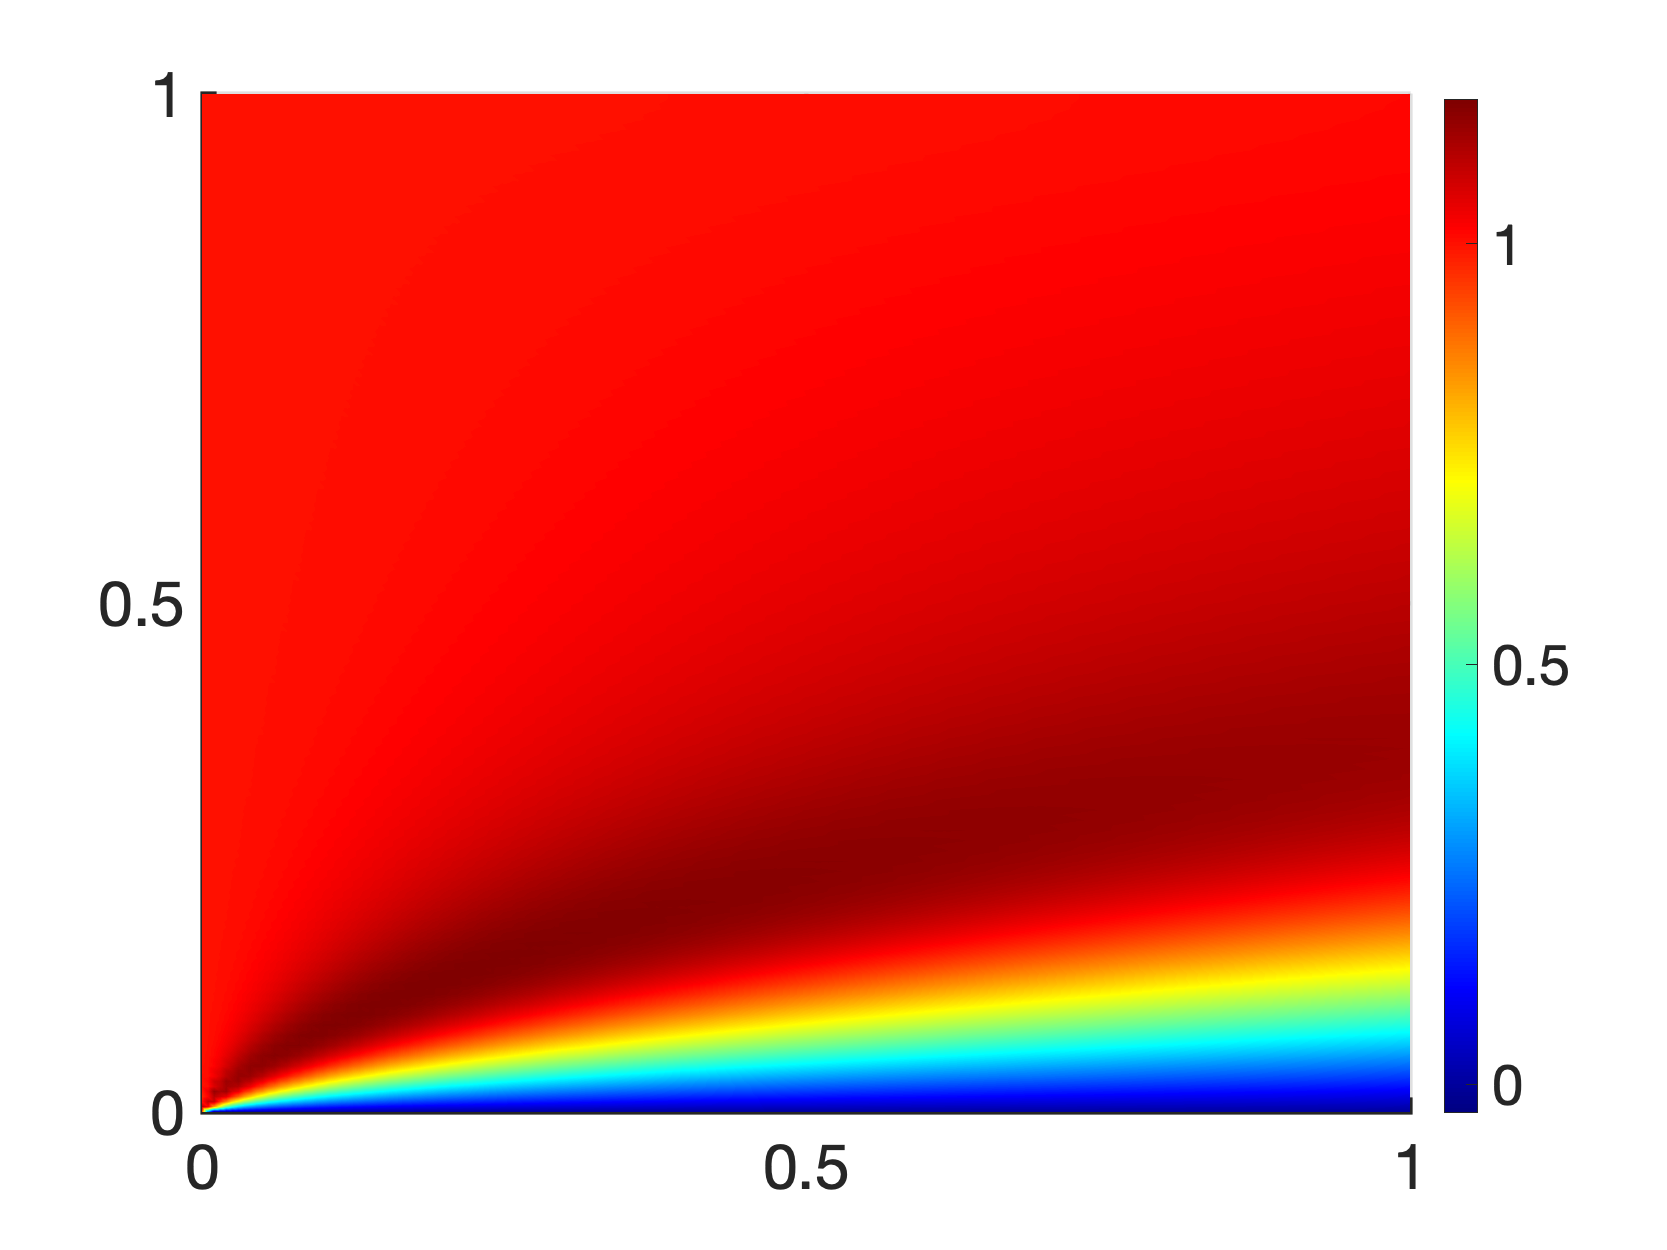
\includegraphics[scale = 0.3]{images/boundary_layer}
  \caption{Flow over a solid surface.}
  \label{fig:boundary_layer}
\end{figure}

\begin{table}
  \centering
  \caption{Errors and the estimated (iterative) convergence rates for the flow over a solid surface.}
  \begin{tabular}{c| cc }
   \hline
  k & $\|e_k\|_\infty$ & $p$
  \\
  \hline
  1 & 1.68e+00  & --  \\
  2 & 6.17e-01  & --  \\
  3 & 1.15e-01  & 1.67 \\
  4 & 4.37e-03  & 1.95 \\
  5 & 1.02e-05  & 1.85 \\
  6 & 5.51e-11  & 2.00 \\
  \hline
  Theoretical && 2
  \end{tabular}
  \label{tab:boundary_layer}
\end{table}

In the last experiment, we consider a curved grid \cite{aalund2019encapsulated} for the incompressible Euler equation (i.e. $\epsilon = 0)$. Both the south and north sides are solid surfaces, where the normal velocity is zero. The west side is an inflow boundary where $u = 1$ and $v = 0$ are specified and at the east side, $p = 0$ is imposed. We change the domain to $\Omega = [-1.5,1.5]\times [0, 0.8]$ and include a smooth bump at the south boundary given by $y(x) = 0.0625e^{-25x^2}$ \cite{bumpgrid} . In \Cref{fig:bump}, the converged solution is illustrated and the estimated iterative convergence rate $p$ is presented in \Cref{tab:bump} for the initial guess $(\un^0;\vn^0;\pn^0) = (1, \dots,1; 0, \dots ,0; 1,\dots 1)$. Again, the results agree well with the theoretical value.
\begin{figure}
 \centering
  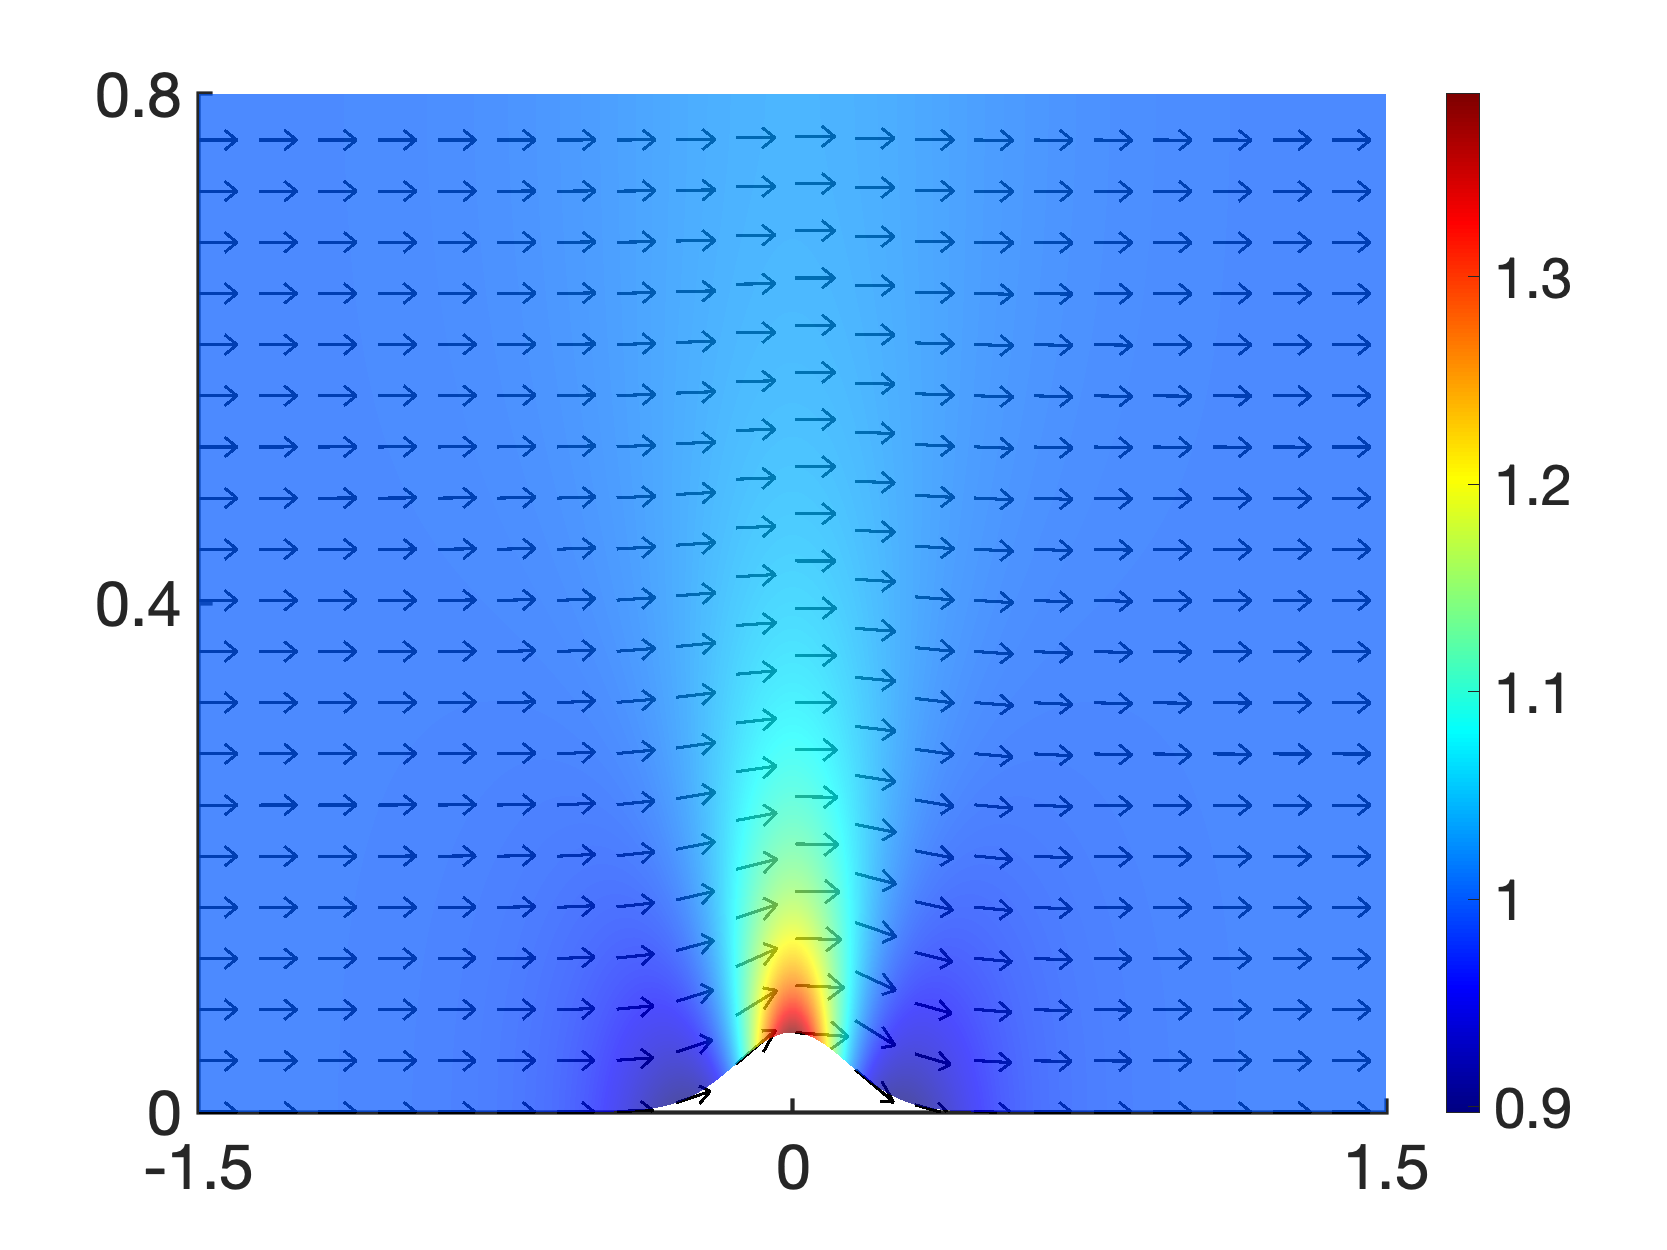
\includegraphics[scale = 0.3]{images/bump.png}
  \caption{Flow over a smooth bump. The plot illustrates the velocity field (arrows) and $\un$ (color figure) at the converged solution.}
  \label{fig:bump}
\end{figure}

\begin{table}
\centering
\caption{Errors and the estimated (iterative) convergence rates for the bump.}
\begin{tabular}{c| cc }
 \hline
k & $\|e_k\|_\infty$ & $p$
\\
\hline
1 &  3.56e+00 & --  \\
2 &  4.91e-01 & --  \\
3 &  1.74e-02 & 1.69 \\
4 &  3.33e-05 & 1.87 \\
5 &  1.55e-10 & 1.96 \\
\hline
Theoretical && 2
\end{tabular}
\label{tab:bump}
\end{table}

  \section{Summary and conclusions}
We derived an explicit expression for the Jacobian of the discretization of the incompressible Euler equations. Due to the use of encapsulated difference operators, the extension to a curved grid is straight forward. Different boundary conditions such as the solid wall, the Dirichlet inflow and pressure outflow conditions have been used and the Jacobian for all these sets of boundary conditions were also presented. Lastly, the numerical method has been illustrated for different cases and also verified by the method of manufactured solutions. 

  \bibliographystyle{unsrt}
  \bibliography{references}
\end{document}
